\documentclass[10pt,a4paper]{article}
\usepackage{graphicx} % Required for inserting images
\usepackage[style=arsclassica]{classicthesis}
\usepackage[dutch]{babel}
\usepackage{amsmath,amssymb,amsfonts}
\usepackage{float,flafter}
\usepackage{hyperref}
\usepackage{inputenc}
\usepackage[margin=2.5cm]{geometry}
\usepackage[margin=2.5cm]{geometry}

\makeatletter
\renewenvironment{equation}{\begin{equation*}}{\end{equation*}}
\makeatother

\begin{document}

\begin{center}
{\Huge\textbf{Samenvatting sterrenstelsel}\par}
\end{center}
\section*{Hoofdstuk 1 (voor de geinteresseerden)}
\section*{1.1 Opening van de deep sky}

\subsection*{1.1.1 Het prille begin}
\begin{itemize}
  \item Extragalactische sterrenkunde is, ondanks de hoge leeftijd van sterrenkunde als wetenschap, \textbf{verbazingwekkend jong}: pas ongeveer \textbf{100 jaar geleden} werden galaxieën als \textbf{extragalactische objecten} erkend en werd aangetoond dat het universum verder reikt dan de Melkweg.
  \item De \textbf{Melkweg} is zichtbaar als een \textbf{witte band} over de hemel: in het \textbf{noordelijk halfrond} enkel op een \textbf{maanloze zomernacht}, in het \textbf{zuidelijk halfrond} \textbf{prominenter} en \textbf{altijd zichtbaar}. Dit verklaart mee waarom ze eeuwenlang mythen en legenden inspireerde.
  \item De oude Grieken beschreven de Melkweg als een \textbf{rivier van melk} (Hera); \textbf{``galaxie''} komt van het Griekse \textbf{gala} (melk). De Romeinen noemden haar \textbf{Via Lactea}.
  \item Grote stap richting extragalactische sterrenkunde: de \textbf{uitvinding van de telescoop (1608)}. \textbf{Galileo (1610)} toonde door de Melkweg te observeren dat de band bestaat uit \textbf{heel veel lichtzwakke sterren} (niet een diffuse ``hemelse vloeistof''), waardoor duidelijk werd dat de Melkweg in de eerste plaats een \textbf{sterrenstelsel} is.
  \item \textbf{Immanuel Kant (1755)}:
  \begin{itemize}
    \item Verklaarde de vlakke structuur van het zonnestelsel via \textbf{zwaartekracht} (samenhouden) en \textbf{geordende rotatie} (niet instorten).
    \item Stelde dat de schijnbare bandstructuur van de Melkweg kan ontstaan als ons stersysteem \textbf{schijf-achtig} is, waarin \textbf{systematische rotatie} de \textbf{zwaartekracht} in evenwicht houdt.
    \item Het centrale vlak heet het \textbf{Galactisch Vlak}; vanuit onze positie binnenin zou een schijf als een \textbf{band langs een grote cirkel} zichtbaar zijn.
    \item Sterren buiten het vlak vergeleek hij met \textbf{kometen}: minder geordend, meer willekeurige banen.
  \end{itemize}
  \item Kant opperde ook de theorie van \textbf{eiland universa}: sommige diffuse deep-sky objecten zouden \textbf{volledige sterrenstelsels} kunnen zijn, vergelijkbaar met de Melkweg maar op grote afstand en met willekeurige inclinaties.
  \item Met het blote oog zijn buiten de Melkweg moeilijk objecten te zien:
  \begin{itemize}
    \item Zuidelijk halfrond: \textbf{Grote} en \textbf{Kleine Magellaanse Wolk} (satellietgalaxieën van de Melkweg).
    \item Noordelijk halfrond: \textbf{Andromeda-galaxie} is het enige externe melkwegstelsel dat met het blote oog goed zichtbaar is (andere mogelijk bij uitzonderlijke omstandigheden).
  \end{itemize}
  \item \textbf{964}: Andromeda en de Grote Magellaanse Wolk werden voor het eerst beschreven door \textbf{Abd-al-Rahman Al Sufi} in het \textit{Boek van de Vaste Sterren}.
  \item Na Galilei's telescoopgebruik werden vele tientallen diffuse deep-sky objecten waargenomen en beschreven; Kant suggereerde dat sommige daarvan \textbf{extragalactische} ``eiland universa'' zijn (achteraf blijkt zijn argumentatie volgens de tekst opvallend accuraat).
\end{itemize}

\subsection*{1.1.2 De 19de eeuw}
\begin{itemize}
  \item Sterkere telescopen leidden eind 18de eeuw tot systematische studie van deep-sky objecten (toen \textbf{``nevels''} genoemd).
  \item \textbf{Charles Messier} publiceerde een belangrijke catalogus met \textbf{110} objecten (galaxieën, planetaire nevels, supernovaresten, bolhopen en open clusters). De Messiernummers worden nog steeds standaard gebruikt (bv.\ \textbf{M31}, \textbf{M51}).
  \item \textbf{William Herschel (1786)}: \textit{Catalogue of Nebulae} met $\sim$\textbf{2400} diffuse objecten (veel ontdekt met \textbf{Caroline Herschel}).
  \item \textbf{John Herschel (1864)}: \textit{General Catalogue of Nebulae and Clusters} met \textbf{5079} objecten.
  \item \textbf{John Dreyer (1888)}: \textbf{New General Catalogue (NGC)} met \textbf{7840} objecten; later uitgebreid met twee \textbf{Index Catalogues (IC)}. \textbf{NGC + IC} blijft een veelgebruikte referentie; veel nabijgelegen galaxieën (niet in Messier) dragen NGC/IC-nummers.
  \item Met betere telescopen kwam de \textbf{aard van nevels} opnieuw ter discussie:
  \begin{itemize}
    \item William Herschel steunde eerst eiland universa (hij kon bolhopen oplossen in sterren), maar dacht later dat sommige nevels (bv.\ Orionnevel, planetaire nevels) waarschijnlijk niet uit sterren bestaan, maar uit een onbekende ``lichtgevende vloeistof''.
    \item John Herschel trok in de jaren 1840 het bestaan van niet-stellaire nevels weer in vraag.
  \end{itemize}
  \item \textbf{Lord Rosse} bouwde de \textbf{Leviathan}-telescoop (diameter \textbf{1,8 m}, grootste van zijn tijd; grootste tot de \textbf{100-inch Mount Wilson telescoop} in 1917). Hij vond dat ``nevels'' niet één homogene klasse zijn, maar in twee \textbf{disjuncte} klassen vallen:
  \begin{itemize}
    \item Detailloze, ellipsvormige lichtvlekjes.
    \item Minder symmetrische objecten met karakteristieke \textbf{spiraalstructuur} $\rightarrow$ \textbf{spiraalnevels} (spiraalstructuur in \textbf{M51} ontdekt in \textbf{1845}).
  \end{itemize}
  \item \textbf{Fotografie}:
  \begin{itemize}
    \item Eerste stappen door Ni\'epce, Daguerre, Talbot; bekendgemaakt in \textbf{1839}.
    \item Astrofotografie experimenteel midden 19de eeuw; vanaf de \textbf{jaren 1880} belangrijk (o.a.\ door de \textbf{droge plaat} in de jaren 1870).
    \item Lange belichtingen maakten zwakkere objecten zichtbaar; één plaat kon duizenden objecten registreren; helderheden konden nauwkeuriger gemeten worden.
    \item Eerste foto van een melkwegstelsel: \textbf{Andromeda (1887)} door \textbf{Isaac Roberts}.
    \item Eind 19de eeuw: grootschalige projecten zoals \textbf{Carte de Ciel} en \textbf{Astrographic Catalogue}.
  \end{itemize}
  \item \textbf{Spectroscopie} (zeker i.c.m.\ fotografie):
  \begin{itemize}
    \item \textbf{William Huggins (1864)}: sommige nevels hebben spectra met \textbf{emissielijnen}, andere hebben een \textbf{stellair} spectrum.
    \item Dit was definitief bewijs voor een fundamenteel verschil: sommige nevels zijn \textbf{gas}, andere zijn \textbf{echte sterclusters}.
    \item Spiraalnevels (bv.\ Andromeda) hadden een \textbf{continu spectrum}; daarom werden ze ook \textbf{``witte nevels''} genoemd.
  \end{itemize}
\end{itemize}

\section*{1.2 Het ontstaan van de extragalactische sterrenkunde}

\subsection*{1.2.1 Het Kapteyn Universum}
\begin{itemize}
  \item \textbf{William Herschel (1785)} probeerde de vorm van de Melkweg te bepalen door sterren te tellen en te catalogeren op helderheid in \textbf{683} hemelgebieden.
  \item Begin 20ste eeuw werd dit ``modern'' herhaald; de meest geavanceerde onderneming stond onder leiding van \textbf{Jacobus Kapteyn}:
  \begin{itemize}
    \item Internationale samenwerking; fotografische opnamen van \textbf{200} gebieden.
    \item Sterren werden geteld en gecatalogeerd per magnitude; ook \textbf{eigenbeweging} werd gemeten.
    \item Met deze databank werd de \textbf{3D verdeling} van sterren afgeleid $\rightarrow$ het \textbf{Kapteyn Universum}.
  \end{itemize}
  \item Kenmerken Kapteyn Universum:
  \begin{itemize}
    \item Ongeveer \textbf{oblate} sterverdeling met \textbf{asverhouding $\sim 5$}.
    \item In de schijf daalt sterdichtheid \textbf{uniform} met toenemende galactocentrische afstand.
    \item Grootte-inschatting: sterdichtheid halveert op \textbf{800 pc}; op \textbf{$\sim 8{,}5$ kpc} is ze nog \textbf{1\%}.
  \end{itemize}
  \item Probleem: de zon kwam uit op \textbf{$\sim 650$ pc} van het Melkwegcentrum; dit was ``verontrustend'' en leek te veel op een soort bevoorrechte positie.
  \item Kapteyn zag een alternatieve verklaring: een \textbf{absorberend interstellair medium} kan verre sterren verduisteren, wat verkeerd kan worden geïnterpreteerd als een afstandseffect (waardoor het lijkt alsof we dicht bij het centrum zitten, ongeacht de echte verdeling).
  \item Hoewel sommige gebieden duidelijk sterk verduisterd zijn, was onbekend of dit losse donkere wolken waren of deel van een algemeen absorberend medium.
  \item Onder de aanname dat verduistering door \textbf{Rayleighverstrooiing} kwam, concludeerde Kapteyn uit helderheidsmetingen op verschillende golflengten dat verduistering \textbf{onbelangrijk} was.
\end{itemize}

\subsection*{1.2.2 Het Grote Debat en de doorbraak}
\begin{itemize}
  \item Niet iedereen accepteerde Kapteyns model. \textbf{Harlow Shapley (1918--1919)} stelde een radicaal ander model voor op basis van \textbf{bolhopen} (sferische sterclusters met $\sim$\textbf{$10^4$ tot $10^6$} sterren):
  \begin{itemize}
    \item Bolhopen zijn over heel de hemel te vinden, maar niet uniform: ze zijn aan beide zijden van het Melkwegvlak ongeveer gelijk verdeeld, maar vertonen een sterke concentratie richting \textbf{Sagittarius} (waar ook de helderste Melkweggebieden liggen).
    \item Shapley redeneerde dat bolhopen een belangrijk structureel element zijn en symmetrisch rond het Melkwegcentrum zouden moeten liggen; de asymmetrie impliceert dat de zon \textbf{niet} dicht bij het centrum ligt.
    \item Via variabele sterren bepaalde hij afstanden: zon $\sim$\textbf{15 kpc} van het centrum van de bolhoopverdeling (en dus waarschijnlijk ook van het Melkwegcentrum).
    \item Hij schatte de Melkweg op $\sim$\textbf{100 kpc} groot (bijna tien keer Kapteyn).
  \end{itemize}
  \item Parallel was er discussie over de \textbf{aard van spiraalnevels}:
  \begin{itemize}
    \item Hypothese 1: onafhankelijke stersystemen op extragalactische afstanden (Kants eiland universa).
    \item Hypothese 2 (Shapley): de Melkweg is zo groot dat het hele universum enkel uit de Melkweg bestaat; spiraalnevels zijn dan een relatief onbelangrijke, gasrijke populatie \textbf{verbonden met de Melkweg}.
  \end{itemize}
  \item \textbf{Spectroscopische aanwijzingen (Slipher)}:
  \begin{itemize}
    \item \textbf{1914}: spectra van enkele spiraalnevels en sommige elliptische nevels zijn verschoven naar langere golflengten (\textbf{roodverschuiving}), geïnterpreteerd via Doppler als wegbeweging met radiale snelheden van \textbf{honderden tot duizenden km s$^{-1}$}.
    \item Deze snelheden zijn veel groter dan bij Melkwegsterren, wat het idee dat ze samen één dynamische entiteit vormen onwaarschijnlijk maakt.
    \item \textbf{1915}: Slipher vond voor \textbf{M104} aanwijzingen voor rotatie met $\sim$\textbf{300 km s$^{-1}$} $\rightarrow$ impliceert enorme massa en dus extragalactische schaal; ook in andere galaxieën (zoals \textbf{M31}) werd ondubbelzinnig rotatie vastgesteld.
    \item Men kon niet verklaren waarom nevels systematisch van de Melkweg weg bewegen; een mogelijke verklaring leek een repulsieve kracht vanuit de Melkweg (wat net weer een connectie impliceerde). De ware betekenis (\textbf{kosmische expansie}) werd volgens de tekst pas \textbf{tien jaar later} blootgelegd.
  \end{itemize}
  \item \textbf{Het Grote Debat (26 april 1920, Washington D.C.)}:
  \begin{itemize}
    \item Publiek debat tussen \textbf{Shapley} (verdedigde vooral zijn Melkwegmodel) en \textbf{Heber Doust Curtis} (sterk in spiraalnevels).
    \item Het was eerder twee korte lezingen ($\sim$30 min) en ze spraken deels naast elkaar, maar het werd legendarisch als symbool van de controverse.
  \end{itemize}
  \item \textbf{Doorbraak (1924)}:
  \begin{itemize}
    \item \textbf{Edwin Hubble} gebruikte de \textbf{100-inch Mount Wilson}-telescoop om een \textbf{cepheïde} in de Andromedanevel te meten.
    \item Cepheïden volgen een periode--lichtkracht-relatie; met periode en schijnbare magnitude kan afstand bepaald worden.
    \item Hubble vond $\sim$\textbf{300 kpc} $\rightarrow$ Andromeda is definitief \textbf{extragalactisch}.
    \item Dit impliceerde dat \textbf{alle witte nevels extragalactische objecten} zijn; sindsdien spreekt men van \textbf{spiraalgalaxieën} i.p.v.\ spiraalnevels.
  \end{itemize}
\end{itemize}

\section*{1.3 Onze Melkweg onder de loep}
\begin{itemize}
  \item De cursus zal per hoofdstuk de Melkweg verder bestuderen: \textbf{sterren, stof, gas en donkere materie} waaruit ze is opgebouwd.
  \item Ondanks dat we in de Melkweg zitten, is een globaal morfologisch beeld moeilijk:
  \begin{itemize}
    \item De Melkweg bevat o.a.\ een \textbf{schijf} van sterren, stof en gas.
    \item Onze positie midden in die schijf maakt waarnemen lastig door \textbf{stofverduistering} en doordat intrinsieke helderheden onzeker zijn door onzekerheid in de correctie voor stofverduistering.
  \end{itemize}
  \item De vroege problematische modellen (Kapteyn vs Shapley-discussie) namen \textbf{stofverduistering niet} mee en leverden zo een fout beeld.
  \item De cursus bespreekt de \textbf{meest recente beschrijving} van de verdeling van sterren, stof en gas.
  \item Veel huidige kennis over vorming en evolutie wordt afgeleid uit \textbf{bewegingspatronen} van componenten, gekoppeld aan de \textbf{chemische samenstelling} van gas en sterren.
  \item De studie van bewegingen is extra moeilijk door onze positie: men moet ook de beweging van de \textbf{Aarde rond de Zon} en de \textbf{Zon rond het sterrenstelsel} in rekening brengen.
\end{itemize}

\section*{Hoofdstuk 2}
\section*{2.1 Telescopen en instrumenten (optisch, NIR, UV) en technieken}

\subsection*{2.1.1 Telescopen en instrumenten in de optische sterrenkunde}
\begin{itemize}
  \item Het elektromagnetische spectrum kan worden ingedeeld in: gammastraling, R\"ontgenstraling, ultraviolette (UV) straling, optische straling (zichtbaar licht), infraroodstraling, millimeterstraling en radiostraling.
  \item Theoretisch is er geen onderscheid tussen deze vormen: het zijn allemaal elektromagnetische golven die zich met de snelheid van het licht voortbewegen. Het verschil is de golflengte $\lambda$ of (equivalent) de frequentie $\nu$, verbonden door
  \begin{equation}
    \lambda = \frac{c}{\nu}
    \tag{2.1}
  \end{equation}
  met $c$ de lichtsnelheid.
  \item In de praktijk is er wel een groot verschil: elk golflengtegebied bevat informatie die meestal in andere gebieden niet of nauwelijks kan worden achterhaald, omdat sterren en gaswolken verschillende temperaturen en chemische samenstellingen kunnen hebben en zich daardoor in verschillende vensters manifesteren.
  \item Het optische venster is het gebied waarin het vermogen van de meeste sterren, inclusief de zon, het grootst is.
  \item Optisch licht bevindt zich ruwweg tussen $350$ en $900$ nm; dit is iets ruimer dan het golflengtebereik van het menselijk oog ($\sim 400$--$700$ nm).
  \item De aardatmosfeer is bijna volledig transparant voor optische straling; daarom kunnen optische telescopen op aarde worden gebouwd. De meeste telescopen (professioneel en amateur) zijn bedoeld voor waarnemingen in het optische gebied.
  \item Technische evolutie: een belangrijke stap was het gebruik van digitale detectoren.
  \item Tot in de jaren 1980 gebruikte men vooral fotografische platen: vrij ongevoelig voor rood licht, niet-lineair en met een redelijk klein bereik.
  \item Tegenwoordig beschikken nagenoeg alle optische telescopen over digitale CCD-detectoren (charged coupled device) met hoge kwantumeffici\"entie over het hele optische gebied en een zeer lineaire respons (voltage evenredig met de invallende straling).
  \item Ook telescopen zelf evolueerden sterk: nagenoeg alle professionele optische telescopen zijn vandaag reflectoren (vroegere refractoren).
  \item Er is een nieuwe generatie 8m-klasse telescopen (o.a.\ Keck op Hawaii en de Very Large Telescope in Chili), wat het lichtvergarend vermogen verhoogt en studie van zwakkere of verder gelegen galaxie\"en toelaat.
  \item Optische observatoria worden op hoge en droge plaatsen gebouwd; belangrijke locaties zijn Chili, Hawaii, het zuidwesten van de VS, Zuid-Afrika, de Canarische Eilanden en Australi\"e.
  \item Een belangrijk criterium (naast lage luchtvochtigheid) is lage seeing: lage atmosferische turbulentie.
  \item Optische sterrenkunde gebeurt ook vanuit de ruimte (o.a.\ Hubble Space Telescope). Vanuit de ruimte is er geen seeing en zijn waarnemingen diffractie-gelimiteerd.
  \item Deze ontwikkelingen leidden tot een revolutie in de sterrenkunde, vooral in extragalactische sterrenkunde en kosmologie.
\end{itemize}

\subsection*{2.1.2 Het nabije infrarood (NIR)}
\begin{itemize}
  \item Het nabije infrarood  is het verlengstuk van het optische venster naar langere golflengten: van ongeveer $1\,\mu$m tot ongeveer $5\,\mu$m.
  \item Waarnemen in het NIR is complexer dan in het optische venster.
  \item Eerste reden: de hemel is relatief veel helderder in het NIR:
  \begin{itemize}
    \item Typische oppervlaktehelderheid van de hemel in Paranal is $\sim 13$ mag arcsec$^{-2}$ op $2\,\mu$m, terwijl galaxie\"en vaak honderden of duizenden keer zwakker zijn.
    \item Tussen $1$ en $2.5\,\mu$m zorgen niet-thermische emissie van de aurora en OH- en O$_2$-emissielijnen voor hoge hemelhelderheid.
    \item Achtergrondstraling is sterk variabel op tijdsschalen van minuten en kan een factor twee verschillen tussen zomer en winter.
    \item Voor $\lambda > 2.5\,\mu$m zijn telescoop en instrumentatie zelf een aanzienlijke bron van achtergrondstraling.
    \item Gevolg: speciale aandacht is nodig om straling van het object te scheiden van straling van de hemel.
  \end{itemize}
  \item Tweede reden: niet het gehele NIR-venster is transparant door de atmosfeer:
  \begin{itemize}
    \item Veel NIR is opaak door water en koolstofdioxide, die NIR-straling gemakkelijk absorberen.
    \item Er zijn slechts enkele vensters waar de atmosfeer transparant is; transparantie hangt af van de atmosfeer.
    \item NIR-waarnemen gebeurt daarom best vanop hoge, droge plaatsen.
    \item Grote observatoria zijn vaak gebouwd op plaatsen geschikt voor zowel optische als NIR-waarnemingen; veel optische telescopen kunnen ook NIR-waarnemen indien de relevante instrumentatie aanwezig is.
  \end{itemize}
  \item Derde reden: detectoren:
  \begin{itemize}
    \item Fotografische platen (optisch, tot jaren 1980) kunnen niet in het NIR gebruikt worden.
    \item Vandaag zijn detectoren elektronisch in beide gebieden, maar technisch anders.
    \item In het NIR kan men geen CCD's gebruiken: CCD's zijn vooral silicium, dat optische fotonen effici\"ent absorbeert, maar niet geschikt is voor de lagere energie van NIR-fotonen.
    \item NIR-detectoren bestaan uit ander materiaal en hebben andere technische karakteristieken voor uitlezen en opslaan, maar werken redelijk analoog.
  \end{itemize}
\end{itemize}

\subsection*{2.1.3 Het UV gebied}
\begin{itemize}
  \item Het ultraviolet (UV) venster heeft golflengten tussen ongeveer $120$ en $3500$ \AA.
  \item UV-sterrenkunde kan, net als NIR-sterrenkunde, als extensie of onderdeel van optische sterrenkunde worden beschouwd: detectoren, spiegels, lenzen en dispersie-elementen zijn gelijkaardig.
  \item Grootste verschil met het optische venster: de aardatmosfeer is transparant voor optische straling en opaak voor UV-straling.
  \item Bijna alle UV-straling wordt geabsorbeerd door ozongas, met grootste concentratie in de ozonlaag; daarom moet UV-waarnemen vanuit de ruimte.
  \item Eerste grote stap: lancering van de International Ultraviolet Explorer (IUE) in 1978 (eerste ruimteobservatorium dat ooit werd gelanceerd).
  \item Bij latere missies namen spectraal bereik, gevoeligheid en spectrale resolutie toe.
  \item Bekende missies: Far-Ultraviolet Spectroscopic Explorer (FUSE) en Extreme Ultraviolet Explorer (EUVE).
  \item Veel missies waren vooral bedoeld om de Melkweg te bestuderen.
  \item Hubble Space Telescope heeft UV-instrumentatie aan boord.
  \item GALEX nam o.a.\ de hele hemel waar in twee UV-banden en is belangrijk voor extragalactische sterrenkunde en kosmologie.
\end{itemize}

\subsection*{2.1.4 Observationele technieken}
\subsubsection*{Fotometrie}

\begin{itemize}
  \item Fotometrie is de eenvoudigste observationele techniek.
  \item Een fotometer bestaat in essentie uit een telescoop en een detector die het vermogen registreert dat door de telescoop wordt opgevangen.
  \item De informatie bestaat uit \'e\'en enkele flux op de golflengte waarop het instrument is ingesteld.
  \item In de optische sterrenkunde wordt fotometrie vooral gebruikt voor sterren, omdat bijna alle sterren behalve de zon puntbronnen zijn.
  \item Snelle en nauwkeurige fotometers zijn handig om fluxvariaties te bestuderen van variabele sterren of dubbelstersystemen.
\end{itemize}

\subsubsection*{Imaging en oppervlaktehelderheid}
\begin{itemize}
  \item Als de resolutie beter is dan de schaal van het object, kan men objecten ruimtelijk oplossen.
  \item In extragalactische sterrenkunde is dit meestal zo: zelfs met een kleine optische telescoop kunnen de meeste nabije galaxie\"en ruimtelijk opgelost worden.
  \item Men kan dan flux meten per positie in het beeldveld (praktisch per pixel).
  \item Elke pixel correspondeert met een ruimtehoek; zo kan men de oppervlaktehelderheid meten: flux per eenheid ruimtehoek.
  \item Het meten van oppervlaktehelderheid van opgeloste objecten heet imaging.
\end{itemize}

\subsubsection*{Wide-field surveys en beam splitters}
\begin{itemize}
  \item Wide-field surveys brengen grote delen van de hemel in beeld door vele opnames aan elkaar te naaien.
  \item Typisch gebruikt men instrumenten met reeksen CCD-camera's in de primaire focus (kleine brandpuntsafstand, groot beeldveld).
  \item Sommige wide-field camera's hebben een beeldveld tot een vierkante graad.
  \item Beam splitters splitsen invallende straling in verschillende kleuren zodat men tegelijk in meerdere banden kan waarnemen.
\end{itemize}

\subsubsection*{Spectroscopie}
\begin{figure}[H]
    \centering
    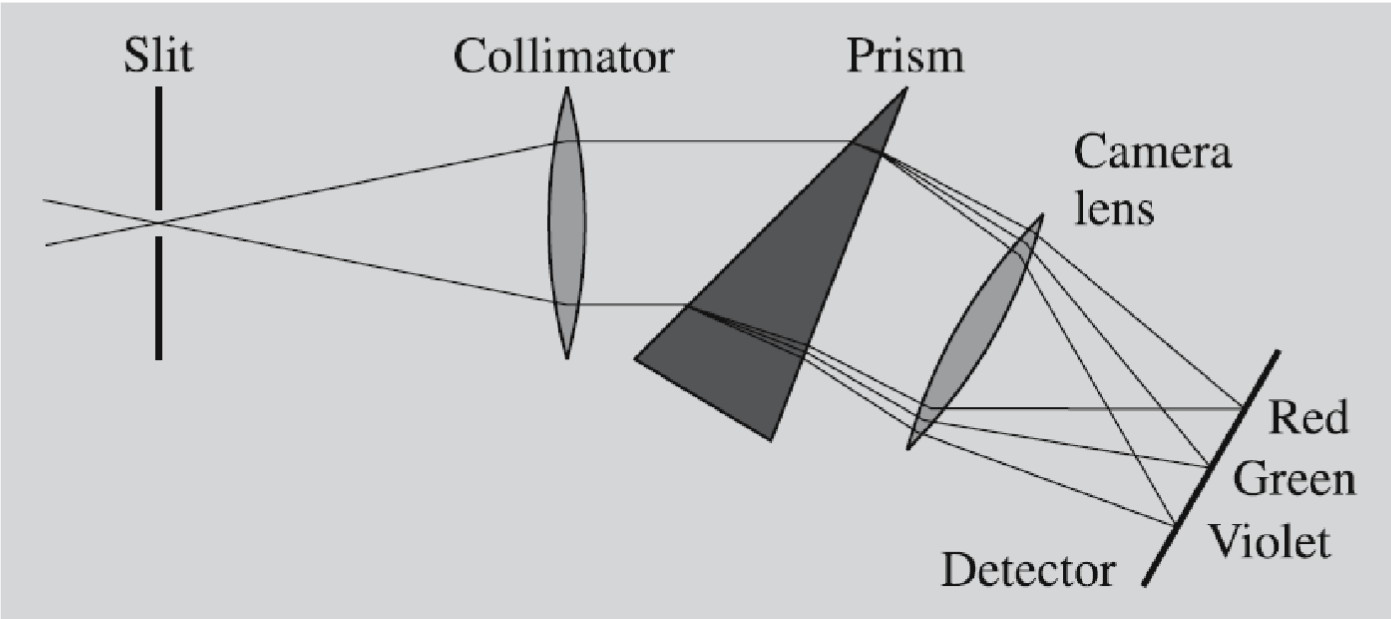
\includegraphics[width=0.5\linewidth]{foto'sH2/fotometrie.png}
    \caption{opstellingsfoto bij spectroscopie}
\end{figure}
\begin{itemize}
  \item Bij spectroscopie gebruikt men een dispersie-element om straling in golflengten te ontbinden en te bestuderen als functie van $\lambda$.
  \item Voorbeeld: een glazen prisma ontbindt wit licht in verschillende kleuren.
  \item Bijna alle professionele telescopen hebben spectroscopen in hun instrumentarium.
  \item Meest gebruikte dispersie-elementen: prisma's, roosters (gratings) of grisms (rooster + prisma).
  \item De keuze hangt af van gewenste resolutie en spectraal bereik; hoge spectrale resolutie gaat meestal ten koste van klein spectraal bereik en lange belichtingstijd.
  \item Een dispersie-element voegt een dimensie toe die gedetecteerd moet worden.
  \item Voor sterren (puntbronnen) bekomt men een 1D-spectrum met $F_\lambda$ als functie van $\lambda$.
  \item Voor melkwegstelsels (2D-objecten) leidt dit conceptueel tot een 3D data cube (2 ruimtelijke + 1 spectrale dimensie), dus een spectrum voor elke positie in het beeldveld.
  \item Omdat er geen optische detectoren bestaan die 3D-informatie kunnen opslaan, is dit een probleem.
\end{itemize}

\subsubsection*{Long-slit spectroscopie}
\begin{figure}[H]
    \centering
    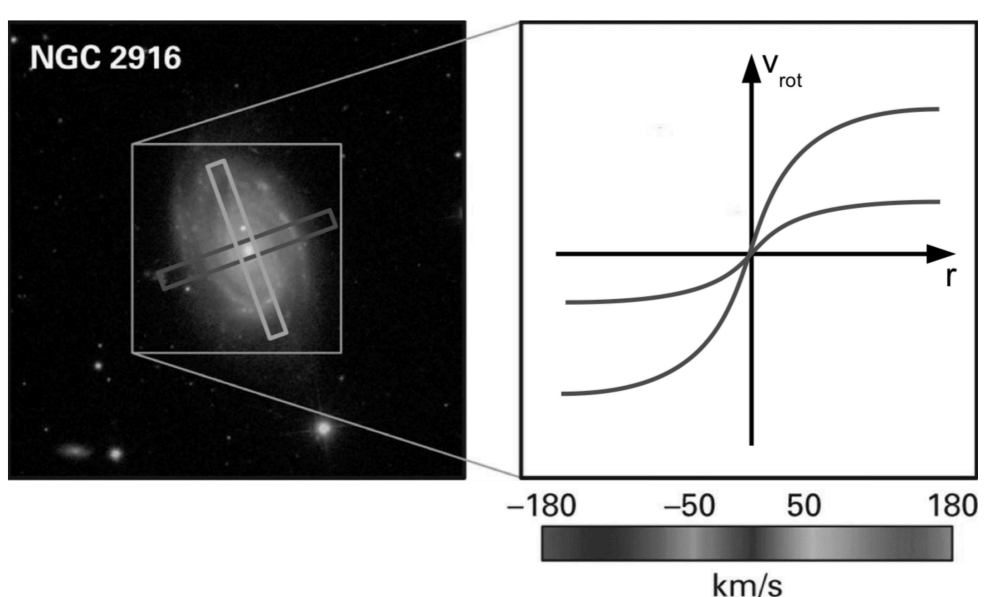
\includegraphics[width=0.5\linewidth]{foto'sH2/Long-Slit.png}
    \caption{long-slit spectroscopie}
\end{figure}
\begin{itemize}
  \item De meest gebruikte oplossing is het inkomende licht beperken tot \'e\'en ruimtelijke dimensie met long-slit spectroscopie.
  \item Men blokkeert alle straling behalve het licht dat door een lange, smalle spleet valt.
  \item Dit licht wordt in loodrechte richting door een dispersie-element gestuurd en op een CCD opgevangen.
  \item Resultaat: een 2D-beeld met \'e\'en ruimtelijke en \'e\'en spectrale dimensie.
  \item Nadeel: men verkrijgt spectra van slechts een beperkt deel van het melkwegstelsel (bv.\ langs de grote as).
\end{itemize}

\subsubsection*{Multi-object spectroscopie}
\begin{figure}[H]
    \centering
    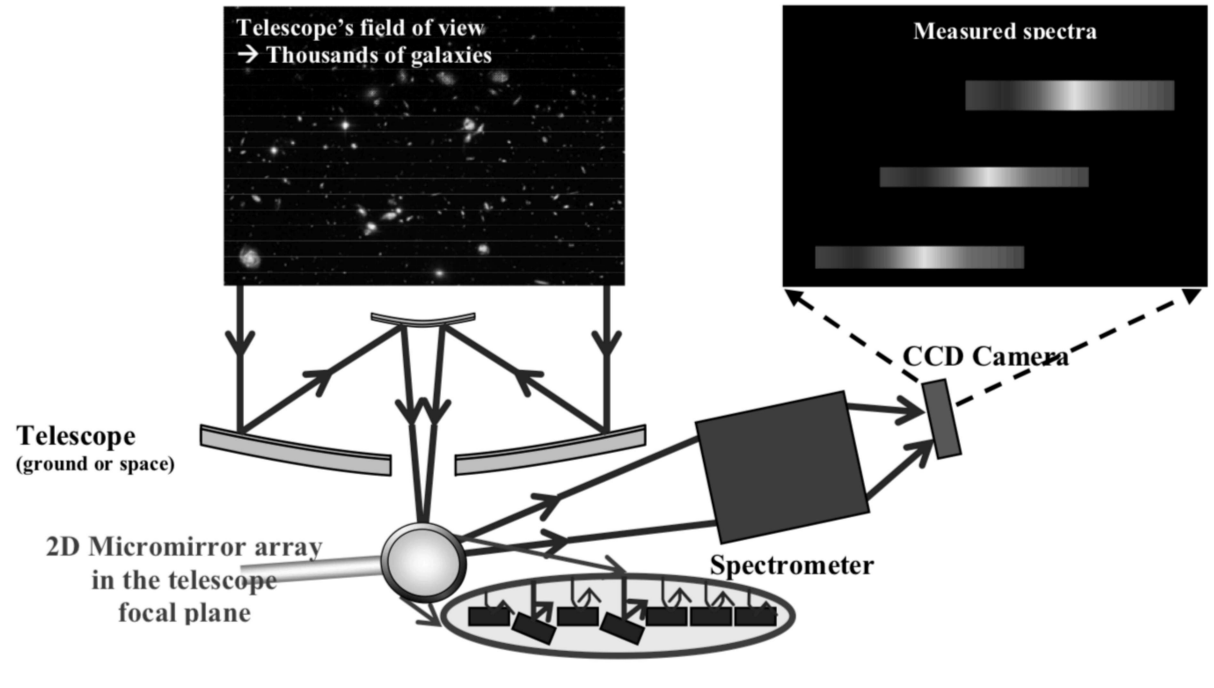
\includegraphics[width=0.5\linewidth]{foto'sH2/pulti-object spectroscopie.png}
    \caption{multi-object spectroscopie}
\end{figure}
\begin{itemize}
  \item Variatie op long-slit: multi-object spectroscopie, nuttig wanneer men in een bepaald gebied spectra van veel objecten wil (bv.\ verafgelegen galaxie\"en in een wide-field survey).
  \item Long-slit zou dan ineffici\"ent zijn.
  \item Oplossing: in plaats van \'e\'en lange slit gebruikt men veel kleine slitjes en een set optische vezels.
\end{itemize}

\subsubsection*{Integral Field Spectroscopy (IFS) en Integral Field Spectroscopy (IFU)}
\begin{figure}[H]
    \centering
    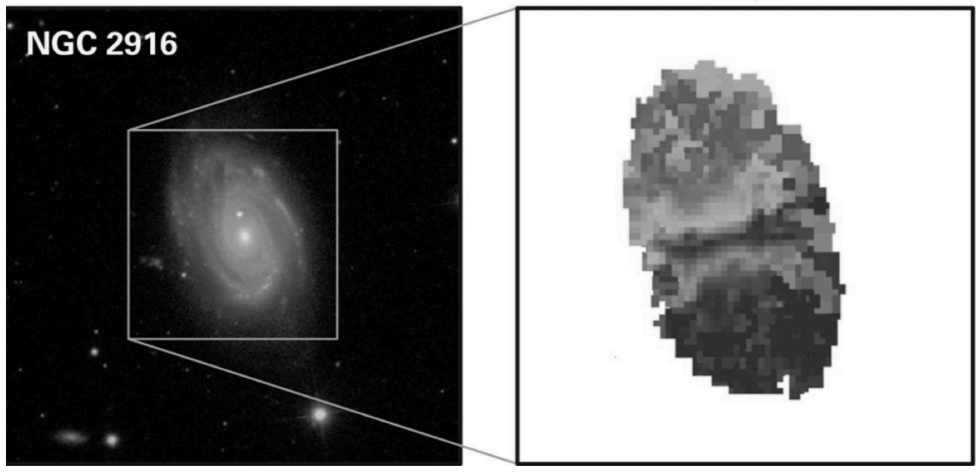
\includegraphics[width=0.5\linewidth]{foto'sH2/IFU.png}
    \caption{IFU spectroscopie}
\end{figure}
\begin{itemize}
  \item Door grotere telescopen en waarnemingen op hoge resolutie werd integral field spectroscopy gestimuleerd.
  \item Een integral field spectrometer (met integral field unit, IFU) combineert imager en spectrometer en maakt 3D-spectroscopy mogelijk: op elke positie in het beeldveld een spectrum.
  \item Men verkrijgt een datacube met 2 ruimtelijke dimensies en 1 spectrale dimensie.
  \item De set-up is uiterst complex; beeldveld wordt opgesplitst via o.a.\ image slicer, microlens array of fibre bundle om uiteindelijk een 3D-datacube op te bouwen.
  \item Terminologie: spaxel = pixelpositie in 2D beeld waarvoor een 1D spectrum beschikbaar is; voxel = datapunt in de 3D datacube (flux op bepaalde golflengte en 2D-positie).
  \item IFU's zijn gebaseerd op bovenstaande technieken (of combinaties) afhankelijk van golflengtegebied, beoogde spectrale resolutie, grootte van beeldveld en objecten.
  \item Integral Field Spectrometers zijn uiterst nuttig voor het bestuderen van de kinematica van sterrenstelsels.
\end{itemize}

\subsection*{2.1.5 Conventies en eenheden}
\begin{itemize}
  \item De (monochromatische) flux $F_\lambda$ gemeten door een waarnemer is de totale hoeveelheid vermogen per eenheid golflengte die op elke oppervlakte-eenheid van de waarnemer aankomt. De eenheid van flux is typisch $\mathrm{W\,m^{-2}\,\text{\AA}^{-1}}$. 
  \item Omdat melkwegstelsels meestal ruimtelijk opgelost zijn, kan men via imaging de monochromatische oppervlaktehelderheid $S_\lambda$ meten. Aangezien oppervlaktehelderheid de waargenomen flux per eenheid ruimtehoek is, is $\mathrm{W\,m^{-2}\,\text{\AA}^{-1}\,arcsec^{-2}}$ een typische eenheid voor oppervlaktehelderheid.
  \item De monochromatische lichtkracht $L_\lambda$ van een object is de hoeveelheid vermogen (energie per tijdseenheid) die een object uitzendt per eenheid golflengte. De eenheid is typisch $\mathrm{W\,\text{\AA}^{-1}}$.
  \item Als we veronderstellen dat een hemellichaam in alle richtingen dezelfde hoeveelheid vermogen uitstraalt, dan zijn lichtkracht en flux verbonden door
  \begin{equation}
    F_\lambda = \frac{L_\lambda}{4\pi d^2}
    \tag{2.2}
  \end{equation}
  waarbij $d$ de afstand is. Indien $d$ gekend is, kan men uit de waargenomen flux de intrinsieke lichtkracht bepalen. In de extragalactische sterrenkunde wordt deze formule ook dikwijls in de andere richting gebruikt: als we de waargenomen flux meten en de intrinsieke lichtkracht kunnen schatten, dan kan men hieruit de afstand bepalen.

  \item Men kan ook de monochromatische flux per eenheid frequentie defini\"eren, $F_\nu$, waarbij ``per eenheid golflengte'' vervangen wordt door ``per eenheid frequentie''. De eenheden voor monochromatische flux, lichtkracht en oppervlaktehelderheid zijn dan typisch $\mathrm{W\,m^{-2}\,Hz^{-1}}$, $\mathrm{W\,Hz^{-1}}$ en $\mathrm{W\,m^{-2}\,Hz^{-1}\,arcsec^{-2}}$.
  \item Het verband tussen beide definities volgt uit
  \begin{equation}
    \left|F_\lambda\,d\lambda\right| = \left|F_\nu\,d\nu\right|
    \tag{2.3}
  \end{equation}
  Deze kan dan als volgt gebruikt worden
  \begin{align*}
      \int_{\lambda_1}^{\lambda_2}F_\lambda(\lambda)d\lambda &=\int^{\nu(\lambda_1)}_{\nu(\lambda_2)}F_{\nu}d\nu\\
      &=\int_{\lambda_2}^{\lambda_1}F_\lambda\frac{d\nu}{d\lambda}d\lambda\\
      &=\int_{\lambda_2}^{\lambda_1}F_\nu\left(-\frac{c}{\lambda^2}\right)d\lambda\\
      &=\int_{\lambda_1}^{\lambda_2}F_{\nu}\frac{\nu}{\lambda}d\lambda
  \end{align*}
  om volgende formules af te leiden
  \begin{equation}
    F_\lambda = \frac{cF_\nu}{\lambda^2} = \frac{\nu^2 F_\nu}{c}
    \tag{2.4}
  \end{equation}
  \begin{equation}
    F_\nu = \frac{\lambda^2 F_\lambda}{c} = \frac{cF_\lambda}{\nu^2}
    \tag{2.5}
  \end{equation}
  Analoge formules gelden uiteraard voor $L_\lambda \leftrightarrow L_\nu$ en $S_\lambda \leftrightarrow S_\nu$.
  \item De verschillende vormen kunnen zonder problemen door elkaar gebruikt worden; vaak worden hybride combinaties gebruikt waarin men bijvoorbeeld $F_\nu$ weergeeft in functie van de golflengte.
  \item Naast monochromatische lichtkracht kan men ook de totale of bolometrische lichtkracht beschouwen:
  \begin{equation}
    L_{\mathrm{bol}} = \int_{0}^{\infty} L_\lambda\,d\lambda
    = \int_{0}^{\infty} L_\nu\,d\nu
    \tag{2.6}
  \end{equation}
  De totale of bolometrische lichtkracht van de zon is $L_\odot = 3.86 \times 10^{26}\,\mathrm{W}$.
\begin{figure}
    \centering
    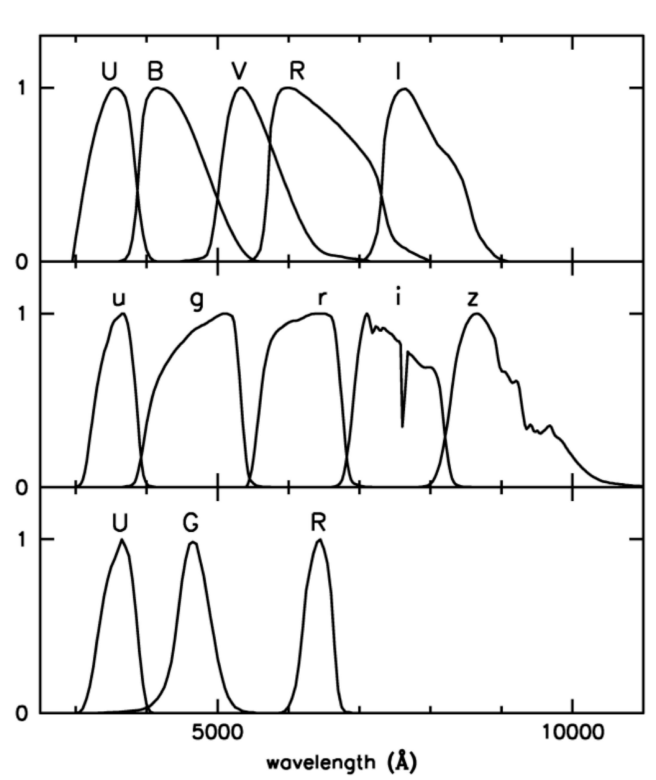
\includegraphics[width=0.4\linewidth]{foto'sH2/filters.png}
    \caption{
    de Johnson--Cousin $UBVRI$ filters (boven) en de SDSS $ugriz$ filters (midden)}
\end{figure}
  \item Het ideaal om via fotometrie of imaging exact de flux te bepalen op een vastgestelde golflengte is niet echt mogelijk; in de praktijk wordt licht in een bepaalde band of filter gedetecteerd.
  \item Elke filter/band wordt gekarakteriseerd door een transmissiecurve $T_\lambda$, die voor elke golflengte $\lambda$ bepaalt welke fractie van de opgevangen straling tot op de detector doordringt.
  \item Wanneer al het licht wordt doorgelaten is $T_\lambda=1$; indien de filter opaak is voor een bepaalde golflengte is $T_\lambda=0$.
  \item De flux $F_X$ in een filter $X$ wordt gedefinieerd als het gewogen gemiddelde van de opgevangen flux:
  \begin{equation}
    F_X \equiv
    \frac{\int_{0}^{\infty} F_\lambda\,T_\lambda(X)\,d\lambda}
         {\int_{0}^{\infty} T_\lambda(X)\,d\lambda}
    \tag{2.7}
  \end{equation}
  \item Er zijn twee soorten filters: breedband- en smalband filters.
  \begin{itemize}
    \item Smalbandfilters hebben een klein golflengtebereik en zijn meestal afgesteld op gebieden met interessante emissielijnen; zo hebben veel telescopen H$\alpha$- of [O~III]-filters rond respectievelijk $6563$ \AA\ en $5007$ \AA.
    \item De meeste optische imagingwaarnemingen gebeuren met breedbandfilters. Die laten veel licht door, waardoor korte belichtingstijden volstaan om een goede signaal-ruis-verhouding te bekomen.
    \item Nadeel van breedbandfilters: ze wassen informatie in hun grote bereik uit (bv.\ vorm van het continuum of aanwezigheid van emissie- of absorptielijnen).
  \end{itemize}

  \item In het optische gebied wordt het Johnson--Cousin systeem gekarakteriseerd door vijf filters: $U$ (ultra-violet), $B$ (blauw), $V$ (visueel), $R$ (rood) en $I$ (infrarood).
  \item Omdat de breedbanden in dit systeem een redelijk grote overlap hebben, is de Johnson--Cousin filterset vanuit astrofysisch oogpunt niet het beste systeem.
  \item De SDSS $ugriz$ filterset (genoemd naar de Sloan Digital Sky Survey) is vanuit astrofysisch oogpunt interessanter en is stilaan bezig de Johnson--Cousin set als standaard te verdringen.
  \item De optische filtersystemen worden uitgebreid naar het nabije infrarood met de $J$, $H$ en $K$ banden, die (ongeveer) samenvallen met de vensters waarin de atmosfeer transparant is.

  \item Behalve fluxen kan men ook lichtkrachten en oppervlaktehelderheden in filterbanden defini\"eren volgens hetzelfde principe.

  \item In de optische sterrenkunde wordt meestal het logaritmische magnitudesysteem gebruikt (oorsprong in het oude Griekenland). De schijnbare magnitude van een ster of galaxie in filter $X$ is
  \begin{equation}
    m_X = -2.5\log\left(\frac{F_X}{F_{X,0}}\right)
    \tag{2.8}
  \end{equation}
  waarbij $F_{X,0}$ het nulpunt (gebaseerd op een set van A0v-sterren) is van filter $X$.
  \item Breedbandoppervlaktehelderheden worden vaak vertaald naar de magnitudeschaal: ze worden genoteerd als $\mu_X$ en uitgedrukt in mag arcsec$^{-2}$.
  \item Verklaring waarom magnitudes gebruikt worden: relatieve metingen zijn (zeker in het optische gebied) veel preciezer dan absolute metingen. Met nauwkeurige waarnemingen kan men relatieve helderheid beter dan $1\%$ meten, wat overeenkomt met
  \begin{equation}
    \Delta m = -2.5\log(1.01) \approx 0.01\,\mathrm{mag}
    \tag{2.9}
  \end{equation}
  Absolute helderheid bepalen is moeilijk; in de praktijk neemt men standaardsterren waar om waarnemingen te ijken.

  \item Net zoals men het helderheidsverschil in dezelfde band kan meten, kan men kleurindices (kleuren) defini\"eren. Een kleur $X-Y$ van een ster of galaxie is het verschil in schijnbare magnitude in twee banden:
  \begin{equation}
    X-Y \equiv m_X - m_Y
    = -2.5\log\left(\frac{F_X}{F_{X,0}}\right)
      + 2.5\log\left(\frac{F_Y}{F_{Y,0}}\right)
    \tag{2.10}
  \end{equation}
  \item Via vergelijking~(2.2) kan dit ook geschreven worden als
  \begin{equation}
    X-Y = -2.5\log\left(\frac{L_X}{L_Y}\right)
          + 2.5\log\left(\frac{F_{X,0}}{F_{Y,0}}\right)
    \tag{2.11}
  \end{equation}
  \item Een kleur komt dus neer op de verhouding van de lichtkracht in twee banden en is een intrinsieke eigenschap van sterren en galaxie\"en. Veelgebruikte kleurindices in het optische gebied zijn $B-V$ en $V-I$.
\end{itemize}
\section*{2.2 Classificatie van melkwegstelsels}

\subsection*{2.2.1 Het Hubble stemvorkdiagram}
\begin{itemize}
  \item Galaxieclassificatie is een zoektocht naar een beschrijving van gemeenschappelijke kenmerken:
  \begin{itemize}
    \item \textbf{Praktisch nut}: individuele objecten kunnen gemakkelijk worden beschreven.
    \item \textbf{Fundamenteel nut}: het bestuderen van de fysische processen die de \textbf{drijvende kracht} zijn van de evolutie van galaxieën.
  \end{itemize}
  
  \item Het eerste echte classificatieschema dat vandaag nog steeds als de  standaard geldt, is het systeem voorgesteld door Edwin Hubble (1889--1953).
\begin{figure}[H]
    \centering
    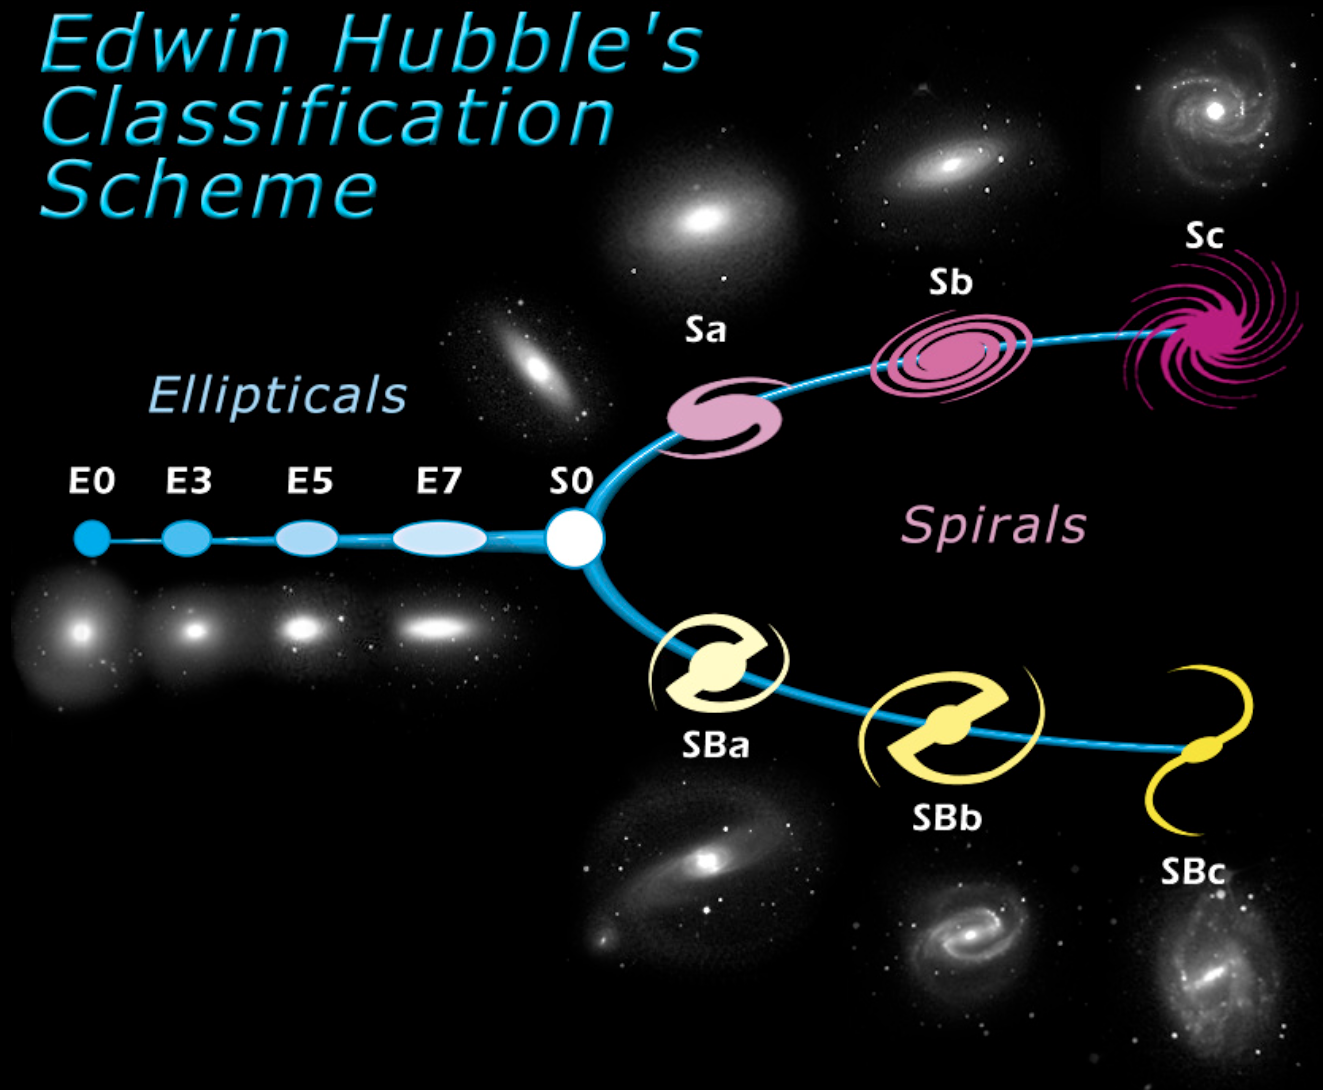
\includegraphics[width=0.5\linewidth]{foto'sH2/hubble twee.png}
    \caption{Hubble-classificatieklassen}
\end{figure}
  \item Het Hubble-classificatieschema wordt traditioneel voorgesteld in de vorm van een stemvork
  \item Het diagram bevat drie grote types van sterrenstelsels, die elk nog onderverdeeld zijn in subklassen.

  \item \textbf{Elliptische galaxieën} (linkerkant van het Hubble-diagram):
  \begin{itemize}
    \item Geen substructuur, behalve een kleine heldere en sterk geconcentreerde nucleus.
    \item Daaromheen: een smooth halo/enveloppe die in alle richtingen continu in helderheid afneemt, zonder duidelijke rand, en gelijkmatig overgaat in de helderheid van de hemel.
    \item Hun vorm op de hemelsfeer is ruwweg ellipsvormig.
    \item De klasse wordt onderverdeeld aan de hand van de schijnbare afplatting.
    \item Een elliptische galaxie wordt geclassificeerd als \textbf{E$j$}, waarbij $j$ de ellipticiteit aangeeft volgens:
    \begin{equation}
      j = 10\left(1-\frac{b}{a}\right)
      \tag{2.12}
    \end{equation}
    met $a$ en $b$ respectievelijk de halve grote en de halve kleine as van de galaxie aan de hemel.
    \item De reeks varieert van \textbf{E0} (ronde galaxieën) tot \textbf{E7}. Elliptische galaxieën met een afplatting sterker dan E7 worden niet waargenomen en bestaan waarschijnlijk niet.
    \item De ellipticiteit is een pover classificatiekenmerk:
    \begin{itemize}
      \item Ten eerste is het \textbf{schijnbaar} en geen intrinsieke eigenschap en zegt het weinig over de inwendige fysica van elliptische galaxieën.
      \item Ten tweede is de schijnbare afplatting \textbf{slecht gedefinieerd}, aangezien de ellipticiteit van elliptische galaxieën vaak verandert naargelang de diepte van het beeld waarmee men de classificatie verricht.
    \end{itemize}
  \end{itemize}

  \item \textbf{Spiraalgalaxieën} (rechtsboven in het Hubble-diagram):
  \begin{itemize}
    \item Gekenmerkt door een centrale lichtconcentratie (de bult) en een schijf met spiraalarmen.
    \item Het aantal spiraalarmen en hun vorm, lengte, regelmatigheid en sterkte kan sterk verschillen van galaxie tot galaxie.
  \end{itemize}

  \item \textbf{Balkspiraalgalaxieën} (rechtsonder in het Hubble-diagram):
  \begin{itemize}
    \item Hebben dezelfde kenmerken en onderverdeling als de spiraalstelsels, maar hebben bovendien een prominente niet-axisymmetrische balk.
  \end{itemize}

  \item Onderverdeling in het oorspronkelijke Hubble-diagram:
  \begin{figure}[H]
      \centering
      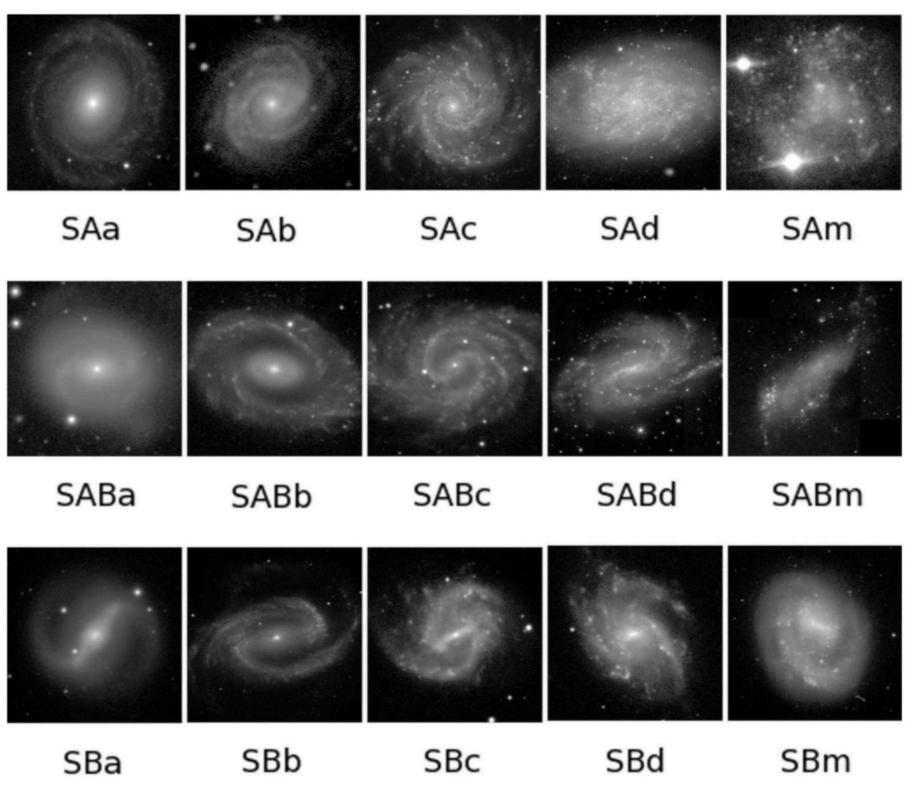
\includegraphics[width=0.5\linewidth]{foto'sH2/onderverdeling.png}
      \caption{onderverdeling visualisatie}
  \end{figure}
  \begin{itemize}
    \item Spiraalgalaxieën: \textbf{Sa, Sb, Sc}, waarbij de grootte van de bult en de karakteristieken van de spiraalarmen bepalend zijn.
    \item Balkspiraalstelsels: analoge onderverdeling in \textbf{SBa, SBb, SBc}.
    \item \textbf{Sa- en SBa-galaxieën}: de bult is dominant; spiraalarmen zijn meestal heel sterk omwonden en redelijk smooth.
    \item \textbf{Sc- en SBc-galaxieën}: veel kleinere bult; spiraalarmen zijn meestal veel meer open en vaak verbrokkeld of met veel substructuur.
    \item Die substructuur kan het gevolg zijn van \textbf{actieve stervormingsgebieden} (armen stralen extra veel licht uit) of van \textbf{donkere stofwolken} (absorberen veel straling).
  \end{itemize}

  \item Later zijn ook de latere types \textbf{Sd, Sm en Im} toegevoegd (waarbij de \textbf{m} staat voor \textbf{Magellaanse}) en hun analogen voor balkspiraalgalaxieën:
  \begin{itemize}
    \item Deze types hebben nauwelijks een centrale bult en de spiraalstructuur is heel open en onregelmatig.
    \item Ook werden tussencategorieën zoals \textbf{Sab} en \textbf{SBcd} toegevoegd aan de reeks.
  \end{itemize}

  \item De overgang tussen spiraalstelsels met en zonder balk wordt op een meer continue manier aangeduid door een tussensoort \textbf{SAB}:
  \begin{itemize}
    \item Spiraalstelsels zonder balk: \textbf{SA}.
    \item Stelsels met een prominente balk: \textbf{SB}.
    \item Tussenklasse: \textbf{SAB}.
  \end{itemize}

  \item In de klassieke Hubble-classificatie kan ook worden aangegeven of de spiraalstructuur in het centrum echt spiraalvormig is of eerder de vorm van een \textbf{ring} heeft:
  \begin{itemize}
    \item Dit geeft de achtervoegsels \textbf{(s)}, \textbf{(r)}, \textbf{(sr)} en \textbf{(rs)}.
    \item Voorbeelden van notatie: \textbf{SA(r)cd} of \textbf{SAB(rs)b}.
  \end{itemize}

  \item Op het punt waar de drie armen samenkomen, bevindt zich de klasse van de lensvormige galaxieën:
  \begin{itemize}
    \item Genoteerd als \textbf{S0} of \textbf{SB0}.
    \item Ze bestaan uit een bult en schijf (en een balkstructuur voor de SB0-types), net als de spiraalgalaxieën, maar er zijn \textbf{geen spiraalarmen} aanwezig.
    \item Ze worden ook nog in enkele subklassen onderverdeeld, naargelang:
    \begin{itemize}
      \item de \textbf{smoothness} van de galaxie,
      \item de \textbf{sterkte van de balk},
      \item het al dan niet voorkomen van één of twee \textbf{ringstructuren}.
    \end{itemize}
    \item Overgangsvormen tussen lensvormige systemen en spiraalgalaxieën, waarin beginnende spiraalstructuur kan worden opgemerkt, worden als \textbf{S0/a} of \textbf{SB0/a} genoteerd.
    \item Er is ook een tussencategorie voor galaxieën die tussen de elliptische en lensvormige vakken vallen; deze worden als \textbf{E/S0} genoteerd.
  \end{itemize}

  \item Opmerking over de herkenbaarheid van lensvormige systemen (S0):
  \begin{itemize}
    \item De klasse van lensvormige systemen is \textbf{niet heel duidelijk herkenbaar}.
    \item Een \textbf{schijf zonder spiraalstructuur} is niet steeds gemakkelijk op te merken, zeker wanneer het stelsel zo georiënteerd is dat we vanop aarde \textbf{loodrecht op de schijf} kijken.
    \item Lensvormige sterrenstelsels met een kleine inclinatie kunnen daardoor gemakkelijk als \textbf{elliptische} galaxieën worden gecatalogeerd.
    \item Moeilijk om in schijven die we op hun kant zien de spiraalstructuur te onderscheiden en te kwantificeren, voor zulke galaxieën is het moeilijk om een onderscheid te maken tussen de \textbf{lensvormige} of \textbf{Sa}-galaxieën.
  \end{itemize}
\end{itemize}
\subsection*{2.2.2 Voor- en nadelen van de Hubble classificatie}
\begin{itemize}
  
  \item \textbf{Nadeel 1: gebaseerd op schijnbare (morfologische) eigenschappen}
  \begin{itemize}
    \item Het stemvorkdiagram is gebaseerd op schijnbare eigenschappen en heeft dus geen fysische achtergrond.
  \end{itemize}

  \item \textbf{Nadeel 2: het systeem omvat enkel de ``normale'' galaxieën}
  \begin{itemize}
    \item Met verbeterde observatietechnieken blijkt dat veel galaxieën nauwelijks of helemaal niet in dit schema passen.
    \item Voorbeelden van categorieën die niet goed passen:
    \begin{itemize}
      \item Elliptische en sferoidale dwerggalaxieën (\textbf{dS0, dE})
      \item Interagerende galaxieën of \textbf{mergers}
      \item Ultra-lichtkrachtige infraroodgalaxieën (\textbf{ULIRGs})
      \item Blauwe compacte dwergen (\textbf{BCDs})
    \end{itemize}
    \item Sommige van deze galaxieën worden ondergebracht bij irregulier galaxieën; andere krijgen het achtervoegsel \textbf{p} van peculiar.
    \item Het aantal galaxieën dat niet in het Hubble diagram past is niet minimaal: elliptische dwerggalaxieën zijn bv.\ een zeer veel voorkomende soort melkwegstelsels.
    \item Ook in het \textbf{vroege heelal} (hoge roodverschuiving) vormt het stemvorkdiagram geen adequate beschrijving van de verschillende types galaxieën.
  \end{itemize}

  \item \textbf{Nadeel 3: verwarrende terminologie (``vroege'' vs ``late'' types)}
  \begin{itemize}
    \item Oorspronkelijk werd aangenomen dat sterrenstelsels evolueren van links naar rechts in het Hubble stemvorkdiagram.
    \item Daarom worden elliptische en lensvormige stelsels vaak als \textbf{vroege types} aangeduid, terwijl spiraalgalaxieën \textbf{late types} zijn.
    \item Ook binnen (balk)spiraalstelsels duidt men de reeks van \textbf{Sa tot Sd} aan als gaande van vroegere naar latere types.
    \item Al snel bleek dat zo’n evolutie \textbf{niet} bestaat.
    \item De benaming is bovendien verwarrend. In elliptische galaxieën is de dominante sterpopulatie vaak oude, koele sterren van het late type, terwijl in de spiraalarmen van spiraalstelsels veel jonge, hete vroeg-type sterren zitten.
  \end{itemize}

  \item \textbf{Nadeel 4: kwalitatief en discreet (niet kwantitatief en niet continu)}
  \begin{itemize}
    \item Het systeem is niet kwantitatief. Er bestaan geen objectief meetbare, kwantitatieve criteria om een sterrenstelsel in een bepaalde klasse onder te verdelen.
    \item Dezelfde galaxieën worden door verschillende auteurs vaak \textbf{verschillend} geclassificeerd.
    \item Classificatie is in het bijzonder moeilijk voor systemen met een \textbf{grote inclinatie}.
    \item Daarnaast is het systeem \textbf{discreet} en niet continu.
    \item Om deze problemen te verhelpen werden de \textbf{Hubble types $T$} ingevoerd:
    \begin{itemize}
      \item Numerieke schaal met stapgrootte $\Delta T = 1$ voor elke overgang tussen twee klassen (bv.\ van Sb naar Sbc).
      \item Spiraal- en balkspiraalgalaxieën van hetzelfde type (bv.\ Sab en SBab) worden samengenomen en hebben $T > 0$:
      \begin{itemize}
        \item Sa: $T=1$, Sab: $T=2$, \dots\ tot $T=9$ voor Sm-galaxieën.
      \end{itemize}
      \item Negatieve waarden van $T$ corresponderen met vroeg-type galaxieën:
      \begin{itemize}
        \item S0/a: $T=0$
        \item Lensvormige galaxieën: $T=-1$ tot $T=-3$
        \item Elliptische galaxieën: $T=-4$ tot $T=-6$
      \end{itemize}
      \item De onderverdeling bij lensvormige en elliptische galaxieën gebeurt op basis van de \textbf{centrale concentratie van het licht}:
      \begin{itemize}
        \item Compacte elliptische galaxieën: $T=-6$
        \item Meer diffuse elliptische melkwegstelsels: $T=-4$
      \end{itemize}
    \end{itemize}
    \item Het Hubble type is handig wanneer we galaxieën \textbf{automatisch} willen classificeren, maar:
    \begin{itemize}
      \item hoewel Hubble types discreet werden ingevoerd, kunnen automatische programma’s een stelsel classificeren als bv.\ $T = 3.56$;
      \item Hubble type is \textbf{kwalitatief} en $T$ is dus niet direct op een meetbare grootheid gebaseerd.
    \end{itemize}
  \end{itemize}

  \item \textbf{Nadeel 5: gebaseerd op optische eigenschappen}
  \begin{itemize}
    \item Het optische venster is slechts een klein deel van het volledige elektromagnetische spectrum; optische waarnemingen bevatten dus maar beperkte informatie vergeleken met multi-golflengte waarnemingen.
  \end{itemize}

  \item \textbf{NIR vs optisch: ander beeld van dezelfde galaxie}
  \begin{itemize}
    \item De NIR-straling van galaxieën  wordt gedomineerd door licht van geëvolueerde rode reuzensterren.
    \item Deze sterren representeren meestal goed de globale stellaire populatie.
    \item NIR-licht wordt bovendien veel minder uitgedoofd door interstellaire stof en geeft daarom vaak een betere schatting van de intrinsieke massaverdeling dan optisch licht.
    \item De spiraalarmen zijn veel minder prominent in NIR-beelden dan in optische opnames.
    \item Een (meestal verwaarloosbare) bijdrage aan NIR-emissie kan ook komen van rode superreuzen, die enkel in stervormingsgebieden voorkomen.
  \end{itemize}

  \item \textbf{UV vs optisch: tracer van recente stervorming}
  \begin{itemize}
    \item UV-straling is voornamelijk afkomstig van de heetste sterren.
    \item Omdat de heetste sterren een zeer korte levensduur hebben, zijn UV-heldere sterren noodzakelijk jong.
    \item UV-straling is dus een tracer voor recente stervorming in melkwegstelsels.
    \item De kosmische achtergrond is vrij laag in het UV-venster, zodat men stervorming met een lage oppervlaktehelderheid relatief gemakkelijk kan detecteren.
    \item Interpretatieprobleem: UV-straling wordt heel efficiënt uitgedoofd door interstellair stof.
    \item Aangezien massale stervorming plaatsvindt in dichte moleculaire wolken die rijk zijn aan interstellair stof, is de UV-flux meestal niet onmiddellijk te converteren naar een maat voor de stervorming.
    \item Analyse van het UV-licht kan wel nuttige informatie leveren over de ruimtelijke verdeling en de chemische samenstelling van het interstellair stof.
  \end{itemize}

  \item \textbf{Multi-golflengte surveys en waarom Hubble toch blijft}
  \begin{itemize}
    \item Tegenwoordig worden  grote all-sky surveys verricht in vele vensters van het spectrum:
    \begin{itemize}
      \item \textbf{UV}: Galaxy Evolution Explorer (\textbf{GALEX}) All Sky Survey
      \item \textbf{optisch}: Sloan Digital Sky Survey (\textbf{SDSS})
      \item \textbf{NIR}: Two Micron All Sky Survey (\textbf{2MASS})
      \item \textbf{MIR en FIR}: Akari All Sky Survey, WISE All Sky Survey
      \item \textbf{radio}: The Arecibo Legacy Fast ALFA Survey (\textbf{ALFALFA}), The VLA Faint Images of the Radio Sky at Twenty-cm (\textbf{FIRST}) survey
    \end{itemize}
    \item Dankzij zulke surveys zal men binnenkort classificatieschema’s kunnen hanteren die gebaseerd zijn op waarnemingen op verschillende golflengten.
    \item Ondanks nadelen blijft het Hubble diagram grotendeels overeind als het standaard classificatiesysteem:
    \begin{itemize}
      \item Een eerste reden is dat het systeem ingeburgerd is.
      \item Voornaamste reden: vele fysische eigenschappen van galaxieën correleren met het Hubble type.
    \end{itemize}
    \item Voorbeelden van correlerende fysische eigenschappen:
    \begin{figure}[H]
        \centering
        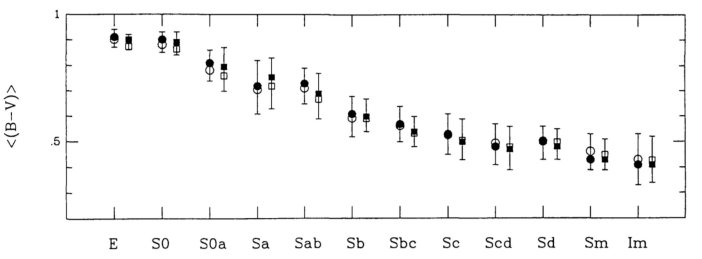
\includegraphics[width=0.5\linewidth]{foto'sH2/corelatie.png}
        \caption{correlatie classificatie klasse en kleur}
    \end{figure}
    \begin{itemize}
      \item Relatieve gasinhoud: $M_{\mathrm{HI}}/L_B$
      \item Massaconcentratie
      \item Kleur 
      \item Spectrale eigenschappen van de stellaire populaties
      \item Chemische abundanties in het interstellaire medium
    \end{itemize}
    \item Hoewel het Hubble classificatiesysteem oorspronkelijk geen fysische achtergrond had, blijkt het achteraf gezien dus wel op fysische gronden te steunen en ons iets te leren over de inwendige structuur van galaxieën.
    \item Dit is uiteindelijk het belangrijkste objectief van classificatie.
  \end{itemize}
\end{itemize}

\subsection*{2.2.3 Classificatie in grote databanken}
\begin{itemize}
  \item Moderne surveys (bv.\ SDSS) bevatten zóveel objecten en spectra dat classificatie ``op zicht'' onhaalbaar wordt; er zijn dus alternatieve methoden nodig.

  \item \textbf{Galaxy Zoo}
  \begin{itemize}
    \item Succesvolle aanpak via het grote publiek (crowdsourcing) om galaxieën te classificeren (o.a.\ SDSS en Hubble Deep Field).
    \item Vrijwilligers krijgen een korte training; elk stelsel wordt door veel mensen geclassificeerd, waardoor het resultaat zelfcorrigerend werkt.
    \item Het project telt $>350\,000$ vrijwilligers en $>60$ miljoen geclassificeerde melkwegstelsels.
  \end{itemize}

  \item \textbf{Automatische classificatie}
  \begin{itemize}
    \item Neurale netwerken leren classificatieregels uit een trainingsset van galaxieën met bekende types.
    \item Tests tonen dat ze statistisch vergelijkbaar kunnen presteren met experts die op zicht classificeren.
  \end{itemize}

  \item \textbf{Kwantitatieve (parametrische) classificatie}
  \begin{itemize}
    \item Doel: een rigoureus systeem op basis van objectief meetbare parameters (niet noodzakelijk gekoppeld aan het Hubble-diagram).
    \item Parameters kunnen uit beelden komen, en eventueel ook uit kleuren of spectra; ze moeten zo objectief mogelijk meetbaar zijn en liefst niet sterk onderling correleren.
    \item Voorbeelden van vaak gebruikte parameters:
    \begin{itemize}
      \item Lichtconcentratie (correleert met Hubble-type; praktisch goed meetbaar).
      \item Asymmetrie (onderscheid ``normale'' vs interagerende/merging stelsels).
      \item Grootte via een diametermaat (bv.\ $D_{25}$-isofoot, komt overeen met de diameter van de isofote met oppervlaktehelderheid 25 mag arcsec$^{-2}$ in de optische B-band).
      \item Smoothness/contrast-parameter $\chi$ (vergelijk origineel en gefit beeld; sterk resolutie-afhankelijk).
    \end{itemize}
  \end{itemize}

  \item Hoewel er vooruitgang is richting fysisch geïnspireerde classificatie, zijn veel schema’s nog optisch gedreven; met nieuwe multi-golflengte databanken zullen spectra en andere golflengten steeds meer worden ingebouwd. Het ultieme classificatiesysteem is dus nog niet bereikt.
\end{itemize}
\section*{Projectie en deprojectie}
\subsection*{2.3.1 Projectie op het vlak van de hemel}
\begin{itemize}
  \item Een typisch model voor een sterrenstelsel bestaat uit een combinatie van componenten. 
  \item Twee relevante grootheden:
  \begin{itemize}
    \item De stellaire emissiviteit $j(\vec{r})$: uitgestraald radiatief vermogen per volume-eenheid en per ruimtehoek.
    \item De intensiteit $I(\vec{r},\vec{k})$ van het stralingsveld: radiatief vermogen per ruimtehoek doorheen een oppervlakte-eenheid loodrecht op richting $\vec{k}$.
  \end{itemize}
  \item Cruciaal verschil: emissiviteit is een \textbf{3D} grootheid, intensiteit is een \textbf{2D} (geprojecteerde) grootheid op het hemelvlak.
  \item Het verband tussen beide is een integratie langs de gezichtslijn:
  \begin{equation}
    I(\vec{r}_{\mathrm{obs}},\vec{k}) = \int_{0}^{\infty} j(\vec{r}_{\mathrm{obs}} + s\vec{k})\,ds
    \tag{2.13}
  \end{equation}
  \item Voor externe galaxieën (schaal $\sim$ kpc) op grote afstand (tientallen Mpc) mogen we de kromming van de hemel lokaal verwaarlozen: de projectie kan als parallel worden beschouwd.
  \item We kiezen een coördinatenstelsel $(x',y',z')$ met $x'y'$ evenwijdig aan het hemelvlak en $z'$ langs de gezichtslijn. Dan wordt:
  \begin{equation}
    I(x',y') = \int_{-\infty}^{+\infty} j(x',y',z')\,dz'
    \tag{2.14}
  \end{equation}

  \item Voor de intrinsieke structuur is een tweede coördinatenstelsel $(x,y,z)$ vaak natuurlijker (bv.\ met symmetrievlak). Projectie vereist dan de transformatie tussen beide stelsels, gekarakteriseerd door kijkhoeken.

\end{itemize}
\subsection*{2.3.2 Projectie in speciale geometrieën}
\begin{itemize}
  \item Een veelgebruikte (geïdealiseerde) veronderstelling is \textbf{axiale symmetrie}. Dan is het handig om over te gaan van cartesische coördinaten $(x,y,z)$ naar cilindrische coördinaten $(\rho,\phi,z)$ met:
  \begin{equation}
    \rho = \sqrt{x^2+y^2}
    \tag{2.15}
  \end{equation}
  en kunnen we de emissiviteit schrijven als $j(\rho,z)$.
  \item In dit geval volstaat voor de overgang tussen $(x,y,z)$ en $(x',y',z')$ de inclinatiehoek $i$ (hoek tussen de gezichtslijn en de symmetrie-as). De transformatie is een rotatie rond de gemeenschappelijke $x=x'$-as:
  \begin{equation}
    \begin{pmatrix}
      x \\ y \\ z
    \end{pmatrix}
    =
    \begin{pmatrix}
      1 & 0 & 0 \\
      0 & \cos i & -\sin i \\
      0 & \sin i & \cos i
    \end{pmatrix}
    \begin{pmatrix}
      x' \\ y' \\ z'
    \end{pmatrix}
    \tag{2.16}
  \end{equation}
  en omgekeerd:
  \begin{equation}
    \begin{pmatrix}
      x' \\ y' \\ z'
    \end{pmatrix}
    =
    \begin{pmatrix}
      1 & 0 & 0 \\
      0 & \cos i & \sin i \\
      0 & -\sin i & \cos i
    \end{pmatrix}
    \begin{pmatrix}
      x \\ y \\ z
    \end{pmatrix}
    \tag{2.17}
  \end{equation}
  \item De projectievergelijking kan dan expliciet worden uitgeschreven als:
  \begin{equation}
    I(x',y') = \int_{-\infty}^{+\infty}
    j\!\left(
      \sqrt{x'^2 + (y'\cos i - z'\sin i)^2},
      \,y'\sin i + z'\cos i
    \right)\,dz'
    \tag{2.18}
  \end{equation}

  \item Een tweede belangrijke speciale symmetrie (als speciaal geval van axiale symmetrie) is \textbf{sferische symmetrie}. Dit is vaak een redelijke eerste-orde benadering voor bijvoorbeeld bolhopen, bulten van spiraalgalaxieën of elliptische galaxieën.
\end{itemize}

\begin{itemize}
  \item Bij sferische symmetrie kan de emissiviteit geschreven worden als $j(\rho,z)=j(r)$ met:
  \begin{equation}
    r = \sqrt{\rho^2+z^2} = \sqrt{x^2+y^2+z^2}
    \tag{2.19}
  \end{equation}
  en analoog (in het geprojecteerde stelsel):
  \begin{equation}
    r = \sqrt{x'^2+y'^2+z'^2}
    \tag{2.20}
  \end{equation}
  \item De projectievergelijking wordt dan:
  \begin{equation}
    I(x',y') = \int_{-\infty}^{+\infty} j(r)\,dz'
    = 2\int_{0}^{\infty} j(r)\,dz'
    \tag{2.21}
  \end{equation}
  \item Door $z'$ te vervangen door $r$ vindt men met
  \begin{equation}
    z' = \sqrt{r^2-(x'^2+y'^2)} \equiv \sqrt{r^2-R^2}
    \tag{2.22}
  \end{equation}
  en
  \begin{equation}
    dz' = \frac{r\,dr}{\sqrt{r^2-R^2}}
    \tag{2.23}
  \end{equation}
  waarbij de geprojecteerde straal op het hemelvlak is
  \begin{equation}
    R = \sqrt{x'^2+y'^2}
    \tag{2.24}
  \end{equation}
  dat de waargenomen intensiteit enkel afhangt van $R$:
  \begin{equation}
    I(x',y') = I(R) = 2\int_{R}^{\infty}\frac{j(r)\,r\,dr}{\sqrt{r^2-R^2}}
    \tag{2.25}
  \end{equation}
  \item De projectie van een sferisch symmetrische sterverdeling levert dus een intensiteitsverdeling met cirkelvormige concentrische isofoten.
  \item Dit kan worden uitgebreid naar \textbf{sferoidale} symmetrie: een systeem heeft een sferoidale verdeling wanneer $j(\rho,z)=j(m)$ met
  \begin{equation}
    m = \sqrt{\rho^2+\frac{z^2}{q^2}}
    \tag{2.26}
  \end{equation}
  waarbij $q$ de intrinsieke asverhouding is. Voor dit geval kan de projectievergelijking worden herschreven tot:
  \begin{equation}
    I(x',y') = I(m') = 2\left(\frac{q}{q'}\right)\int_{m'}^{\infty}\frac{j(m)\,m\,dm}{\sqrt{m^2-m'^2}}
    \tag{2.27}
  \end{equation}
\end{itemize}
\begin{itemize}
  \item Bij projectie van een sfero\"idale emissiviteit op het hemelvlak zijn de isofoten concentrische gelijkvormige ellipsen.
  \item De waargenomen asverhouding $q'$ hangt niet af van de functionele vorm van $j$, maar enkel van de inclinatie $i$ en de intrinsieke asverhouding $q$:
  \begin{equation}
    m'=\sqrt{q^2\sin^2 i+\cos^2 i}
    \tag{2.28}
  \end{equation}
  \item Een analoog resultaat geldt ook voor ellipso\"idale massaverdelingen (niet noodzakelijk axiaal-symmetrisch) met:
  \begin{equation}
    m=\sqrt{x^2+\frac{y^2}{p^2}+\frac{z^2}{q^2}}
    \tag{2.29}
  \end{equation}
  waarbij de isofoten opnieuw goed benaderd worden door concentrische ellipsen en de waargenomen asverhouding bepaald wordt door de intrinsieke asverhoudingen en de kijkrichting.
\end{itemize}

\section*{2.4 Morfologische modellen voor melkwegstelsels}
\begin{itemize}
  \item Een eerste stap in de studie van sterrenstelsels is een morfologische beschrijving: men fit een eenvoudig geïdealiseerd model (met enkele parameters zoals schaal en vorm) aan observaties.
  \item Zulke modellen zijn nuttig omdat ze:
  \begin{itemize}
    \item de basiseigenschappen van een galaxie samenvatten in een klein aantal parameters;
    \item toegepast op grote samples kunnen dienen voor geautomatiseerde classificatie;
    \item een eenvoudig, maar bruikbaar ``inputmodel'' leveren voor studies van bv.\ dynamica, stabiliteit en effecten van stof op fotometrie.
  \end{itemize}
\end{itemize}
\subsection*{2.4.1 Elliptische galaxieën}

\begin{itemize}


  \item Voor elliptische stelsels veronderstelt men sferische symmetrie: waargenomen intensiteitsverdeling $I(R)$ cirkelsymmetrisch en kunnen overgangsformules tussen $j(r)$ en $I(R)$ uit sectie 2.3 gebruikt worden.

  \item \textbf{Vaucouleurs-profiel (R$^{1/4}$-wet)}
  \begin{itemize}
    \item Observaties tonen dat $\mu(R)$ vaak bijna lineair is als functie van $R^{1/4}$.
    \item Het profiel kan geschreven worden als:
    \begin{equation}
      \mu(R)=\mu_e+8.3268\left[\left(\frac{R}{R_e}\right)^{1/4}-1\right]
      \tag{2.31}
    \end{equation}
    \item Met het verband $\mu=-2.5\log I + C$ ($C$ een nulpuntsconstante) volgt een equivalente vorm in intensiteit:
    \begin{equation}
      I(R)=I_e\exp\!\left[-7.66924\left(\left(\frac{R}{R_e}\right)^{1/4}-1\right)\right]
      \tag{2.34}
    \end{equation}
    \item Hier werkt $R_e$ als schaallengte en werken $\mu_0$, $I_e$, $I_0$ als normalisatie.
    \item Totale lichtkracht:
    \begin{equation}
      L=2\pi\int_0^\infty I(R)\,R\,dR
      \tag{2.35}
    \end{equation}
    en voor dit model:
    \begin{equation}
      L=0.01058\,I_0R_e^2=22.61\,I_eR_e^2
      \tag{2.36}
    \end{equation}
    \item De constante $7.66924$ is zo gekozen dat $R_e$ de half-licht straal is:
    \begin{equation}
      L(R)=2\pi\int_0^R I(R')R'\,dR',\qquad L(R_e)=\frac{L}{2}.
      \tag{2.37--2.38}
    \end{equation}
  \end{itemize}

  \item \textbf{Exponentieel profiel}
  \begin{itemize}
    \item Niet alle elliptische stelsels volgen een Vaucouleurs-profiel. Voor elliptische dwerggalaxieën (en vaak ook bulten) geeft een exponentieel profiel soms een betere fit:
    \begin{equation}
      I(R)=I_0\exp\!\left(-\frac{R}{h}\right)
      \tag{2.40}
    \end{equation}
    \item Via (2.35) is de totale lichtkracht:
    \begin{equation}
      L=2\pi I_0h^2
      \tag{2.41}
    \end{equation}
    \item De effectieve straal volgt uit de half-licht definitie en is:
    \begin{equation}
      R_e=1.67835\,h,
      \tag{2.42}
    \end{equation}
    zodat:
    \begin{equation}
      I(R)=I_0\exp\!\left[-1.67835\left(\frac{R}{R_e}\right)\right].
      \tag{2.43}
    \end{equation}
  \end{itemize}

  \item \textbf{S\'ersic-profiel}
  \begin{itemize}
    \item Het S\'ersic-model beschrijft een continue overgang tussen exponentieel en Vaucouleurs:
    \begin{equation}
      I(R)=I_0\exp\!\left[-b_m\left(\frac{R}{R_e}\right)^{1/m}\right],
      \tag{2.44}
    \end{equation}
    met $m$ de concentratie-index en $b_m$ zo gekozen dat $R_e$ opnieuw de half-licht straal is.
    \item Voor $0.5<m<10$ geldt een nauwkeurige benadering:
    \begin{equation}
      b_m \approx 2m-0.324.
      \tag{2.45}
    \end{equation}
    \item Totale lichtkracht weer via (2.35):
    \begin{equation}
      L=\frac{2\pi m}{b_m^{2m}}\Gamma(2m)\,I_0R_e^2,
      \tag{2.46}
    \end{equation}
  \end{itemize}

  \item \textbf{Centrale profielen: Nuker-model}
  \begin{itemize}
    \item Hoge-resolutie data tonen dat de centrale oppervlakthelderheid vaak niet naar een eindige waarde convergeert en dat eenvoudige Vaucouleurs/S\'ersic-profielen daar niet volstaan.
    \item Daarom gebruikt men voor centrale profielen het Nuker-model:
    \begin{equation}
      I(R)=2^{(\beta-\gamma)/\alpha}I_b
      \left(\frac{R}{R_b}\right)^{-\gamma}
      \left[1+\left(\frac{R}{R_b}\right)^{\alpha}\right]^{(\gamma-\beta)/\alpha}.
      \tag{2.47}
    \end{equation}
    \item $R_b$ markeert de overgang tussen een binnenste en buitenste machtswet-regime; $I_b$ is de intensiteit op $R_b$.
    \item Uit steekproeven volgt dat de meest lichtkrachtige elliptische galaxieën vaak een kern (afvlakking naar het centrum) hebben, terwijl minder lichtkrachtige elliptische galaxieën meestal geen kern hebben.
    \item De grens tussen beide ligt rond $L_V \approx 2\times 10^{10}L_\odot$ of $M_V\approx -21.7$.
    \item Lichtkrachtige elliptische galaxieën hebben hoge Sersic-waarde ($m>4$), terwijl dwerggalaxieën een lage Sersic-waarde hebben ($m\approx1$).
  \end{itemize}

  \item \textbf{$\gamma$-modellen (analytische emissiviteit)}
  \begin{itemize}
    \item De profielen hierboven hebben geen analytische emissiviteit en zijn dus niet eenvoudig analytisch te deprojecteren.
    \item Een bruikbare familie met eenvoudige emissiviteit zijn de $\gamma$-modellen:
    \begin{equation}
      j(r)=\frac{3-\gamma}{4\pi}\,\frac{La}{r^{\gamma}(a+r)^{4-\gamma}},
      \tag{2.48}
    \end{equation}
    met $a$ schaallengte, $L$ totale lichtkracht, en $\gamma$ een hellingsparameter.
    \item $L$ volgt direct uit integratie in 3D:
    \begin{equation}
      L=\int j(\vec{r})\,d\vec{r}
      \tag{2.49}
    \end{equation}
    en bij sferische symmetrie:
    \begin{equation}
      L=4\pi\int_0^\infty j(r)r^2\,dr.
      \tag{2.50}
    \end{equation}
    \item Voor $\gamma=0,\frac{1}{2},\ldots,\frac{5}{2}$ kan de geprojecteerde intensiteit
    \begin{equation}
      I(R)=2\int_R^\infty \frac{j(r)r\,dr}{\sqrt{r^2-R^2}}
      \tag{2.51}
    \end{equation}
    analytisch worden uitgerekend. Dit maakt de $\gamma$-modellen ook interessant als testmodellen in stellaire dynamica.
  \end{itemize}

  \item \textbf{Van cirkels naar ellipsen: isofoten op het hemelvlak}
  \begin{itemize}
    \item Reële elliptische galaxieën zijn niet sferisch: in eerste orde zijn hun isofoten concentrische, gelijkvormige ellipsen met waargenomen asverhouding $q'$.
    \item Men kan sferische modellen vaak toch blijven gebruiken door $R$ te vervangen door een ``elliptische straal'':
    \begin{equation}
      m'=\sqrt{x'^2+\frac{y'^2}{q'^2}}.
      \tag{2.52}
    \end{equation}
    \item Voor de effectieve straal gebruikt men dan doorgaans het geometrisch gemiddelde van halve grote en kleine as ($X_e$ en $Y_e$):
    \begin{equation}
      R_e=\sqrt{X_eY_e}=\sqrt{q'}\,X_e.
      \tag{2.53}
    \end{equation}
  \end{itemize}

  \item \textbf{Afwijkingen van perfecte ellipsen: disky en boxy}
  % Aanvulling bij sectie 2.4.1: boxy/disky isofoten (vervolg)

\begin{itemize}
  \item Isofoten van elliptische galaxieën zijn meestal goed te benaderen door ellipsen, maar vertonen vaak kleine systematische afwijkingen:
  \begin{itemize}
    \item \textit{disky}: isofoten zijn iets ``uitgetrokken'' langs de grote as;
    \item \textit{boxy}: isofoten zijn ``hoekiger'' met relatief meer licht in de hoeken.
  \end{itemize}

  \item Deze afwijkingen worden gekwantificeerd t.o.v.\ de best-passende ellips. Men kan die referentie-ellips parametriseren als
  \begin{equation}
    x' = a\cos t
    \tag{2.54}
  \end{equation}
  \begin{equation}
    y' = b\sin t
    \tag{2.55}
  \end{equation}
  met $a$ en $b$ de halve grote en kleine as, en $t$ de parameter langs de ellips.

  \item Definieer vervolgens $\Delta r(t)$ als de (radiale) afstand tussen de echte isofote en de referentie-ellips. Deze afwijking kan worden ontbonden in een Fourier-reeks:
  \begin{equation}
    \Delta r(t) = \sum_{k=3}^{\infty} a_k\cos kt + b_k\sin kt
    \tag{2.56}
  \end{equation}
  (de som start bij $k=3$ omdat de best-passende ellips zo gekozen is dat termen $k=0,1,2$ al ``weggefit'' zijn).

  \item In de praktijk is vooral de $a_4$-term belangrijk:
  \begin{itemize}
    \item $a_4>0 \Rightarrow$ \textit{disky} (afwijking het grootst op de assen).
    \item $a_4<0 \Rightarrow$ \textit{boxy} (afwijking het grootst tussen de assen; hoekiger).
  \end{itemize}

  \item Het onderscheid boxy/disky correleert met andere structurele eigenschappen:
  \begin{itemize}
    \item Boxy elliptische galaxieën zijn typisch lichtkrachtiger dan disky elliptischen en zijn gemiddeld helderder in radio- en Röntgengebied.
    \item Uit interne kinematica blijkt dat disky galaxieën doorgaans sneller roteren.
  \end{itemize}

  \item Sommige auteurs suggereren dat de $a_4$-parameter (boxiness/diskiness) fysisch informatiever is dan de klassieke afplatting en daarom als extra (of alternatieve) classificatieparameter voor elliptische stelsels kan dienen.
  \item Dit leidt tot een verfijning van het Hubble-stemvorkdiagram waarbij elliptische galaxieën soms worden opgesplitst in boxy en disky subfamilies, en waarbij ook een verband wordt gelegd met de overgang naar lensvormige (S0) stelsels 
\end{itemize}
\end{itemize}
\subsection*{2.4.2 Spiraalgalaxieën}
\begin{itemize}
  \item Spiraalgalaxieën kunnen worden gezien als een samenstelling van meerdere componenten (schijf, bult, balk, nucleus, spiraalarmen, lens, halo, \dots). Voor ``normale'' spiralen zijn, wat de sterren betreft, vooral de \textit{schijf} en de \textit{centrale bult} de belangrijkste componenten; andere structuren leveren een kleinere bijdrage of kunnen als verstoringen op deze basiscomponenten worden beschouwd.

  \item Voor een eenvoudig model van een sterschijf vertrekt men bij voorkeur vanuit de intrinsieke 3D-structuur. Vaak neemt men aan dat de emissiviteit in radiale en verticale richting kan worden gescheiden:
  \begin{equation}
    j(\rho,z)=f(\rho)\,g(z)
    \tag{2.57}
  \end{equation}
  \item De radiale structuur $f(\rho)$ kan men bepalen uit face-on (of kleine inclinatie) stelsels; de verticale structuur $g(z)$ uit edge-on stelsels. In de praktijk bemoeilijkt interstellair stof de interpretatie van edge-on optische beelden sterk (Figuur 2.19); waarnemingen in het nabije infrarood zijn daarom vaak geschikter.

  \item \textbf{Dubbel-exponentieel schijfmodel}
  \begin{itemize}
    \item Klassiek model waarbij de emissiviteit zowel radiaal als verticaal exponentieel afneemt:
    \begin{equation}
      j(\rho,z)=j_0\exp\!\left(-\frac{\rho}{h}-\frac{|z|}{h_z}\right)
      \tag{2.58}
    \end{equation}
    \item Totale lichtkracht:
    \begin{equation}
      L = 2\pi\int_0^\infty \rho\,d\rho \int_{-\infty}^{+\infty} j(\rho,z)\,dz
      = 4\pi j_0 h^2 h_z
      \tag{2.59}
    \end{equation}
  \end{itemize}

  \item \textbf{Alternatief: isotherme verticale verdeling}
  \begin{itemize}
    \item Een ander model neemt een isotherme verdeling in de verticale richting:
    \begin{equation}
      j(\rho,z)=j_0\exp\!\left(-\frac{\rho}{h}\right)\operatorname{sech}^2\!\left(\frac{z}{z_0}\right)
      \tag{2.60}
    \end{equation}
    met totale lichtkracht:
    \begin{equation}
      L = 4\pi j_0 h^2 z_0
      \tag{2.61}
    \end{equation}
  \end{itemize}

  \item \textbf{Projectieprobleem bij algemene inclinatie}
  \begin{itemize}
    \item Voor beide 3D-schijfmodellen is de geprojecteerde intensiteit $I(x',y')$ in het algemeen niet analytisch te schrijven voor willekeurige inclinatie (enkel in exact face-on of exact edge-on bestaan eenvoudige uitdrukkingen).
  \end{itemize}

  \item \textbf{Limiet: oneindig dunne exponentiële schijf}
  \begin{itemize}
    \item Waarnemingen tonen dat schijven typisch sterk afgeplat zijn: $h/h_z \sim 6$--$12$. Dit motiveert een nog eenvoudiger model door de limiet $h_z\to 0$ te nemen bij vaste $h$ en $L$.
    \item Door (2.58) en (2.59) te combineren kan men schrijven:
    \begin{equation}
      j(\rho,z)=\frac{L}{4\pi h^2 h_z}\exp\!\left(-\frac{\rho}{h}-\frac{|z|}{h_z}\right)
      \tag{2.62}
    \end{equation}
    en in de limiet $h_z\to 0$ volgt een Dirac-delta beschrijving:
    \[
      j(\rho,z)=\frac{L}{2\pi h^2}\exp\!\left(-\frac{\rho}{h}\right)\delta(z).
    \]
    \item Dit model heeft als voordeel dat de projectie een eenvoudige vorm krijgt. Gebruikmakend van de axiaal-symmetrische projectieformule (2.18) kan men afleiden dat:
    \begin{equation}
      I(x',y') = \frac{L}{2\pi h^2 \cos i}\,
      \exp\!\left[-\frac{1}{h}\sqrt{x'^2+\frac{y'^2}{\cos^2 i}}\right]
      \tag{2.64}
    \end{equation}
    \item Dit wordt meestal geschreven als:
    \begin{equation}
      I(x',y')=I(m')=I_0\exp\!\left(-\frac{m'}{h}\right)
      \tag{2.65}
    \end{equation}
    met
    \begin{equation}
      I_0=\frac{L}{2\pi h^2\cos i},
      \tag{2.66}
    \end{equation}
    en de ``elliptische'' straal
    \begin{equation}
      m'=\sqrt{x'^2+\frac{y'^2}{\cos^2 i}}.
      \tag{2.67}
    \end{equation}
    \item De isofoten zijn in dit model gelijkvormige ellipsen en de waargenomen asverhouding is:
    \[
      q'=\cos i.
    \]
  \end{itemize}

  \item \textbf{Gecorrigeerde centrale helderheid (face-on)}
  \begin{itemize}
    \item Vaak gebruikt men als parameter niet de waargenomen centrale intensiteit, maar de face-on gecorrigeerde centrale intensiteit:
    \begin{equation}
      I_0^c=\frac{L}{2\pi h^2}=I_0\cos i
      \tag{2.68}
    \end{equation}
    \item De intensiteitsverdeling kan dan worden geschreven als:
    \begin{equation}
      I(m')=\frac{I_0^c}{\cos i}\exp\!\left(-\frac{m'}{h}\right)
      \tag{2.69}
    \end{equation}
    \item In magnitude-eenheden:
    \begin{equation}
      \mu(m')=\mu_0^c + 2.5\log(\cos i) + 1.087\left(\frac{m'}{h}\right).
      \tag{2.70}
    \end{equation}
  \end{itemize}
\end{itemize}

\section*{Hoofdstuk 9}
\section*{9.1 Het meten van de stellaire kinematica}
\begin{itemize}
  \item Uit de volledige fase-ruimte $(\vec{r},\vec{v})$ kunnen we van externe sterrenstelsels in de praktijk slechts een beperkt aantal grootheden afleiden: de positie op de hemel en de snelheid langs de gezichtslijn.
  \item Dat betekent dat van de zes mogelijke fase-ruimtedimensies er slechts drie rechtstreeks toegankelijk zijn: twee posities op de hemel $(\theta,\phi)$ en de line-of-sight snelheid $v_{los}$.
  \item De studie van de stellaire kinematica steunt daarom op spectroscopie: uit Doppler-verschuivingen van absorptie- of emissielijnen wordt informatie over de beweging van sterren en gas afgeleid.
\end{itemize}

\subsection*{9.1.2 Line-of-sight velocity distribution (LOSVD)}
\begin{itemize}
  \item Een spectraal kenmerk met rustgolflengte $\lambda_0$ verschuift door de radiale snelheid van een ster naar
  \begin{equation}
    \Delta\lambda = \lambda-\lambda_0 = \frac{v_{los}}{c}\,\lambda_0
    \tag{9.1}
  \end{equation}
  \item In termen van de logaritmische snelheidsvariabele $u=c\ln\lambda$ is die verschuiving bijna recht evenredig met $v_{los}$:
  \begin{equation}
    \Delta u = c\ln\left(\frac{\lambda}{\lambda_0}\right)
    = c\ln\left(1+\frac{v_{los}}{c}\right)
    \approx v_{los}
    \tag{9.2}
  \end{equation}
  \item Wanneer we in een bepaalde richting door een sterrenstelsel kijken, dragen sterren met verschillende snelheden elk hun eigen Doppler-verschuiving bij. Het gemeten spectrum is daardoor niet enkel verschoven, maar ook verbreed.
  \item De LOSVD $F(v_{los})$ wordt zo gedefinieerd dat $F(v_{los})\,dv_{los}$ de fractie sterren geeft met snelheden tussen $v_{los}$ en $v_{los}+dv_{los}$ die bijdragen aan het geobserveerde spectrum.
  \item Hebben de sterren in het sterrenstelsel hetzelfde spectrum $S(u)$, dan geldt:
  \begin{equation}
    G(u)\propto \int F(v_{los})S(u-v_{los})\,dv_{los}
    \Leftrightarrow G(u)\propto F(u)\otimes S(u)
    \tag{9.3}
  \end{equation}
  waarbij $G(u)$ het gecombineerde spectrum is.
  \item Via de relatie tussen convolutie en Fourier-transformatie geldt dan dat
  \begin{equation}
    \tilde{F}(k)\propto \frac{\tilde{G}(k)}{\tilde{S}(k)}
    \tag{9.4}
  \end{equation}
  \item Lijkt gemakkelijk, is het niet:
    \begin{itemize}
      \item Spectrum is een som van spectra van meerdere sterren en dus meerdere types sterren.
      \item Hoge kwaliteit spectroscopische data zijn nodig.
      \item Ruis wordt uitvergroot door deling.
    \end{itemize}
\end{itemize}
\subsection*{9.1.3 Kinematische parameters}
\begin{itemize}
  \item LOSVD is moeilijk in zijn geheel af te leiden, daarom worden vaak eigenschappen gekarakteriseerd. Enkele eenvoudige eigenschappen zijn:
  \begin{itemize}
    \item gemiddelde snelheid:
    \begin{equation}
      \bar{v}_{los}=\int v_{los}F(v_{los})\,dv_{los}
      \tag{9.5}
    \end{equation}
    \item snelheidsdispersie:
    \begin{equation}
      \sigma^2_{los}=\int (v_{los}-\bar{v}_{los})^2F(v_{los})\,dv_{los}
      \tag{9.6}
    \end{equation}
  \end{itemize}
  \item Er wordt een standaardgedaante opgesteld voor LOSVD waarin parameters worden gebruikt; het meest courante model is een gaussiaanse:
  \begin{equation}
  F(v_{los})=\frac{1}{\sqrt{2\pi}\sigma_{los}}\exp\left(-\frac{(v_{los}-\bar{v}_{los})^2}{2\sigma_{los}^2}\right)
  \tag{9.7}
  \end{equation}
  \item Meestal zijn we geinteresseerd in de vorm van de LOSVD. Deze is namelijk niet altijd gaussisch; er kunnen afwijkingen in zitten die informatie kunnen geven over de kinematische structuur.
  \item Meerdere parameters zijn nodig, we introduceren de Gauss-Hermite-reeks:
  \begin{equation}
  F(v_{los})\propto\left(1+\sum_{k=3}^nh_kH_k\left(\frac{v_{los}-\bar{v}_{los}}{\sigma_{los}}\right)\right)\exp\left(-\frac{(v_{los}-\bar{v}_{los})^2}{2\sigma_{los}^2}\right)
  \tag{9.8}
  \end{equation}
  Deze wordt vaak afgebroken na de vierde term, zodat mogelijke parameters $h_3$ (skewness), $h_4$ (kurtosis), $\sigma^2_{los}$ en $\bar{v}_{los}$ zijn.
\end{itemize}
\section*{9.2 Het fundamentele vlak (FV)}
\subsection*{9.2.1 De Faber-Jackson-relatie}  
\begin{itemize}
  \item Uit Dopplerverschuiving van een galaxie kunnen de radiale snelheid en de snelheidsdispersie $\sigma_0$ van de galaxie worden afgeleid.
  \item Omdat de centrale gebieden van de galaxie helderder zijn dan de randgebieden, is $\sigma_0$ ongeveer gelijk aan de snelheidsdispersie langs de centrale kijklijn.
  \item Deze dispersie is een belangrijke parameter:
  \begin{itemize}
    \item Ze is een maat voor de massa van een galaxie: hoe massiever de galaxie, hoe sneller de sterren erin bewegen.
    \item Ze staat in relatie met de lichtkracht van een galaxie:
    \begin{equation}
    \frac{L_V}{2\times10^{10}L_\odot}\approx\left(\frac{\sigma_0}{200\,\mathrm{km/s}}\right)^4
    \tag{9.9}
    \end{equation}
  \end{itemize}
\end{itemize}
\subsection*{9.2.2 Het fundamentele vlak}
\begin{itemize}
  \item De schatter in de Faber-Jackson-relatie kan m.b.v. de effectieve straal geelimineerd worden via de relatie $L=2\pi \langle I\rangle_eR_e^2$:
  \item In de driedimensionele ruimte gevormd door ($\log R_e$, $\log \sigma_0$, $\log \langle I\rangle_e$) liggen elliptische galaxieën op een vlak, het fundamentele vlak:
  \begin{equation}
  \log(R_e)=\alpha \log(\sigma_0)+\beta \log(\langle I\rangle_e)+\Gamma
  \quad \Longleftrightarrow \quad
  R_e\propto \sigma_0^\alpha \langle I\rangle_e^\beta
  \tag{9.10}
  \end{equation}
  \item Door elliptische galaxieen in clusters te onderzoeken, kan het FV bepaald worden. Door dan te vergelijken met andere FV's, kunnen standaardwaarden voor $\alpha$, $\beta$ gevonden worden:
  \begin{equation}
  \alpha=1.24\pm0.07 \quad \text{en} \quad \beta=-0.82\pm0.02
  \tag{9.11}
  \end{equation}
  $\Gamma$ verschilt ook niet veel van cluster tot cluster. Het fundamentele vlak is universeel.
\end{itemize}
\subsection*{9.2.3 Fysieke betekenis van het fundamentele vlak}
\begin{itemize}
  \item Voor een fysische interpretatie te kunnen geven, moeten de waarneembare grootheden verbonden worden aan fysische grootheden.
  \item Een sterrenstelsel in evenwicht voldoet aan het viriaaltheorema:
  \begin{equation}
  2T_{tot} + W_{tot}= 0
  \tag{9.12}
  \end{equation}
  \item $\langle R\rangle$ en $\langle v^2\rangle$ worden gedefinieerd als:
  \begin{equation}
  W_{tot}=-\frac{GM^2}{\langle R\rangle}
  \quad \text{en} \quad
  T_{tot}=\frac{1}{2}M\langle v^2\rangle
  \tag{9.13}
  \end{equation}
  \item Er gelden ook de volgende relaties:
  \begin{equation}
  k_R\langle R\rangle = R_e
  \quad \text{en} \quad
  k_v\langle v^2\rangle = \sigma_0^2
  \tag{9.14}
  \end{equation}
  met parameters $k_R$ en $k_v$ reflecterend respectievelijk de morfologische en kinematische structuur van elliptische galaxieën.
  \item We definieren ook de massalichtverhouding $\Upsilon$ als:
  \begin{equation}
  \Upsilon = \frac{M}{L} = \frac{M}{2\pi \langle I\rangle_e R_e^2}
  \tag{9.15}
  \end{equation}
  \item Combineren we alles, dan vinden we een uitdrukking voor $R_e$:
  \begin{equation}
  R_e = \frac{k_S}{\Upsilon}\sigma_0^2\langle I\rangle_e^{-1}
  \tag{9.16}
  \end{equation}
  met $k_S = \frac{1}{2\pi Gk_Rk_v}$:
  \begin{equation}
  k_S = \frac{1}{2\pi Gk_Rk_v}
  \tag{9.17}
  \end{equation}
  \item Vergelijken we deze relatie met (9.10), dan vinden we:
  \[
  \frac{k_S}{\Upsilon} \propto \sigma_0^{\alpha-2}\langle I\rangle_e^{\beta+1}
  \]
  Deze uitdrukking beschrijft de helling van het fundamentele vlak; die heeft twee oorzaken:
  \begin{itemize}
    \item Variatie van de massalichtverhouding $\Upsilon$.
    \item Variatie van de structurele parameters $k_R$ en $k_v$.
  \end{itemize}
\end{itemize}

\begin{itemize}
  \item Om de helling van het FV te verklaren, moet de variatie van $\Upsilon$ onderzocht worden. We hebben:
  \[
  \sigma_O=k^{-\frac{1}{2}}R_e^{\frac{1}{2}}\langle I\rangle_e^{\frac{1}{2}}\Upsilon^{\frac{1}{2}}
  \]
  zodat
  \[
  \Upsilon \propto k_S\langle I\rangle_e^{-\frac{1}{2}-\frac{2\beta}{\alpha}-\frac{1}{\alpha}}=k_SL^{\frac{1}{\alpha}-\frac{1}{2}}
  \]
  waarin in de tweede stap $\alpha$ en $\beta$ werden ingevuld en zo $\langle I\rangle_e$ wegviel. Mogelijke verklaringen voor deze helling zijn:
  \begin{itemize}
    \item Elliptische galaxieen zijn structureel homologisch: $k_S$ is constant en $\Upsilon$ varieert met de lichtkracht $L$.
    \[
    \Upsilon \propto L^{\frac{1}{\alpha}-\frac{1}{2}} \text{of equivalent} \Upsilon \propto M^{\frac{2-\alpha}{2+\alpha}}
    \]
    Meest massieve lichtkrachtige galaxieen hebben een hogere $\Upsilon$; dit is een samenspel van factoren:
    \begin{itemize}
      \item Massieve sterren hebben grote metalliciteit $\implies$ $\Upsilon$ neemt toe bij blauwere golflengtes.
      \item Massieve galaxien hebben meer donkere materie.
    \end{itemize}
    \item Elliptische galaxieen zijn structureel niet-homologisch: $k_S$ varieert met de lichtkracht $L$ en $\Upsilon$ is constant.
  \end{itemize}
  \item FV heeft nog een praktisch nut:
  \begin{itemize}
    \item $\sigma_0$ en $\langle I\rangle_e$ zijn afstandsonafhankelijk terwijl $R_e$ afstandsafhankelijk is.
    \item Bij meten van deze drie parameters kan de galaxie in het FV geplaatst worden en kan de afstand tot de galaxie bepaald worden uit de conversie van $R_e$ van kPc naar boogseconden.
  \end{itemize}
\end{itemize}
\section*{9.3 Ruimtelijk opgeloste stellaire kinematica}
\begin{itemize}
  \item M.b.v. 3D-spectroscopie kan een kinematische kaart gemaakt worden waarop elke pixel zijn eigen LOSVD-parameterwaarde ($\bar{v}_{los}, \sigma_{los}, h_3, h_4$) heeft.
  \item Hiermee kunnen orbitaalbanen van sterren in de galaxie bepaald worden, of kan hiermee de massaverdeling in een galaxie bepaald worden.
\end{itemize}
\subsection*{9.3.1 Anisotropie in elliptische galaxieen}
\begin{itemize}
\item De meeste kinematische profielen zijn redelijk regelmatig:
\begin{itemize}
  \item $\sigma_{los}$ en $h_4$ zijn gewoonlijk symmetrisch.
  \item $\bar{v}_{los}$ en $h_3$ zijn gewoonlijk antisymmetrisch.
\end{itemize}
\item $\bar{v}_{los}$ is negatief aan de ene kant en positief aan de andere kant, of omgekeerd $\implies$ rotatie. Dit is consistent met rotatie als oorzaak van afplatting.
\item De maat van afplatting ($\epsilon$) wordt bepaald door de verhouding van $\bar{v}_{los}$ en $\sigma_{los}$. Als een elliptische galaxie concentrisch ellipsoidisch is en een isotrope snelheidsdispersie heeft, wordt de relatie gegeven door:
\[
\frac{\bar{v}_{los}}{\sigma_{los}}\approx\sqrt{\frac{\epsilon}{1-\epsilon}}
\]  
\item De meeste elliptische galaxieen voldoen niet aan deze relatie, rotatie is geen voledige verklaring voor afplating $\implies$ anisotropie (het niet constant zijn van $\sigma$ binnen een galaxie) is ook een belangrijke factor in de afplatting van elliptische galaxieen.
\end{itemize}
\subsection*{9.3.2 Dynamische modellering van elliptische galaxieen}
\begin{itemize}
  \item Uit data willen we een dynamisch model opbouwen dat aan data gefit kan worden.
  \item stellaire dynamica is de intristieke beweging van van de sterren; stellaire kinematica is de beweging van de sterren zoals we die waarnemen (projectie op het hemelvlak).
  \item We willen de distributiefunctie $f(\bar{r}, \bar{v})$ achterhalen; deze geeft aan hoeveel sterren op positie $\bar{r}$ en met snelheid $\bar{v}$ bewegen.
  \item Ook de waargenomen dynamica aan de hemel moet volgen uit de projectie van $f(\bar{r}, \bar{v})$ op het hemelvlak.
  \item Het verband tussen LOSVD en distributiefunctie is gegeven door:
  \[
  F(v_los, x', y') = \int^{-\infty}_{+\infty} \int \int f(\bar{r}, \bar{v})\,dv_{x'}dv_{y'}dz'
  \]
  De buitenste integraal is over de gezichtslijn, de binnenste integralen zijn over het vlak in de snelheidsruimte loodrecht op de gezichtslijn.
  \item Waargenomen rotatiesnelheid en snelheidsdispersie vinden we ook:
  \[
  \bar{v}_{los}(x', y')=\int^{-\infty}_{+\infty} \int \int \int f(\bar{r}, \bar{v})\,d\vec{v}_{los}dz'
  \]
  \[
  \sigma^2_{los}(x', y')=\int^{-\infty}_{+\infty} \int \int \int (v_{los}-\bar{v}_{los})^2f(\bar{r}, \bar{v})\,d\vec{v}_{los}dz'
  \]
  \item De meest populaire methode om een dynamisch model te fitten aan waarnemingen is de Schwarzschild-methode:
  \begin{itemize}
    \item Voor gegeven potentiaal wordt een groot aantal banen berekend.
    \item Uit deze banen kan de tijd die een ster op een bepaalde positie doorbrengt en de gezichtslijnsnelheid die hij dan heeft, worden afgeleid.
    \item Het model volgt dan uit de superpositie van deze banen.
    \item Zie cursus P250 onderaan voor analyse van opbouw van model op deze manier.
  \end{itemize}
  \item Huidige state-of-the-art dynamische modelleringen van elliptische galaxieen zijn SAURON en ATLAS3D.
  \item Deze maken gebruik van 3D-spectroscopiedata en de Schwarzschild-methode.
  \item M.b.v. deze methodes werd duidelijk dat er twee vroege klassen aan galaxien zijn:
  \begin{itemize}
    \item fast rotators: deze zijn snel roterend, hebben een disk-achtige
    \item slow rotators: deze zijn langzaam (of niet) roterend, hebben een meer spheroidale structuur
  \end{itemize}
\end{itemize}
\subsection*{9.3.3 De dynamische opwarming van spiraalgalaxieen}
\begin{itemize}
  \item Het is observationeel moeilijk stelaire kinematica in spiraalgalaxieen te meten:
  \begin{itemize}
    \item ze zijn lichtzwaker in vergelijking met elliptische galaxieen.
    \item  De gemiddelde snelheidsdispersie van de sterren is redelijk laag.
  \end{itemize} 
  \item hoge spectrale resolutie nodig + lage oppervlaktehelderheid van schijfgalaxieen $\implies$ lange belichtingstijden nodig.
  \item Ze zijn dynamisch koude objecten: het grootste deel van de kinetische energie zit in geordende beweging en weinig in willekeurige beweging ($\bar{v}_{los}>>\sigma_{los}$) $\implies$ sterren bewegen dus bijna in cirkelvormige banen.
  \item Willekeurige bewegingen kunnen ons iets vertellen over de evolutie van spiraalgalaxieen: hoe ouder de sterren, hoe groter hun snelheidsdispersie.
  \item Verschillende processen zijn verantwoordelijk voor opwarming van sterrenschijven (willekeurige bewegingen):
  \begin{itemize}
    \item Verstoring van massaverhogingen
    \begin{itemize}
      \item Voornamelijk efficiënt in het geval van de schijf.
      \item signatuur: voornamelijk in de schrijf $\implies$ $\sigma_R>\sigma_z$
    \end{itemize}
    \item Verstrooiing van moleculaire wolken
    \begin{itemize}
      \item gaswolk kan botsen en kinetische energieafgeven aan een ster.
      \item signatuur: Stochastisch proces dat willekeurige bewegingen in alle richtingen verhoogt $\implies$ $\sigma_R\approx\sigma_z$
    \end{itemize}
    \item Interactie met satellieten (andere galaxieen die rond de beschouwde galaxie bewegen)
    \begin{itemize}
      \item Efficiënt als botsing frontaal is.
      \item signatuur: Verticale snelheidsdispersie neemt toe $\implies$ $\sigma_R<\sigma_z$
    \end{itemize}
  \end{itemize}
\end{itemize}
\subsection*{9.3.5 kinematische ontkoppede kernen}

\section*{9.4 Ons melkweg onder de loep}
\subsection*{9.4.1 kinematica van de melkweg}

\end{document}